% -*- mode: latex; mode: visual-line; fill-column: 9999; coding: utf-8 -*-
%
% For submission to 'Concurrency and Computation: Practice and Experience'
% http://www.cc-pe.net/journalinfo/index.html 
% 
% ACM classifiers https://www.acm.org/publications/computing-classification-system/1998
% D.1.3 Concurrent Programming (parallel)
% J.2 PHYSICAL SCIENCES AND ENGINEERING
%

\documentclass[LATO1COL]{WileyNJD-v2}
\usepackage[numbers,super,sort&compress]{NJDnatbib}

%%%%%%%%%%%%%%%%%%%%%%%
%% Wiley bibliography styles
%%%%%%%%%%%%%%%%%%%%%%%
% included with AMA option
%%\bibliographystyle{WileyNJD-AMA}
%
% use home-grown BST file with author-year capabilities, implementing
% subset of AMA as in https://wol-prod-cdn.literatumonline.com/pb-assets/assets/15320634/amaguide-1509470359000.pdf
% and derived from WileyNJD-AMA
\bibliographystyle{WileyNJD-CCPE}

\makeatletter
\renewcommand{\@biblabel}[1]{\quad#1.}
\makeatother

% fix doi (not sure how to properly enable it in my bst)
\usepackage{hyperref}
\renewcommand{\doi}[1]{doi: \href{https://doi.org/#1}{#1}}

%------------------------------------------------------------

\usepackage{graphicx}
\usepackage{caption}
\usepackage{subcaption}
\usepackage{amsmath}
\usepackage{amssymb}
\usepackage{amsthm}
\usepackage{color}
\usepackage{ifpdf}
\usepackage{booktabs} % For formal tables
\usepackage{listings}
%\setcopyright{rightsretained}

\newcommand{\up}{\vspace*{-1em}}
\newcommand{\upp}{\vspace*{-0.4em}}
\newcommand{\uppp}{\vspace*{-0.2em}}

\usepackage{hyperref}
\usepackage{float}
\usepackage[utf8]{inputenc}
\usepackage{multirow}
\usepackage{rotating}
\usepackage{setspace}
\usepackage{paralist}
\usepackage{makecell}
\usepackage{moresize}
\setlength{\textfloatsep}{5pt}
\usepackage{tabularx}
\usepackage{algorithm}
\usepackage{algpseudocode}

\usepackage{url}
\usepackage{booktabs}
\usepackage{listings}
\usepackage{paralist}
\usepackage{wrapfig}
\usepackage{multirow}
\usepackage{ifpdf}
\usepackage{xspace}
\usepackage{keyval}
\usepackage{color}
\usepackage{nicefrac}
\usepackage{float}

\theoremstyle{definition}
\newtheorem{definition}{Definition}[section]

\definecolor{listinggray}{gray}{0.95}
\definecolor{darkgray}{gray}{0.7}
\definecolor{commentgreen}{rgb}{0, 0.4, 0}
\definecolor{darkblue}{rgb}{0, 0, 0.4}
\definecolor{middleblue}{rgb}{0, 0, 0.7}
\definecolor{darkred}{rgb}{0.4, 0, 0}
\definecolor{brown}{rgb}{0.5, 0.5, 0}

\usepackage[normalem]{ulem}
\def\cyanuwave{\bgroup \markoverwith{\lower3.5\p@\hbox{\sixly \textcolor{cyan}{\char58}}}\ULon}
\def\reduwave{\bgroup \markoverwith{\lower3.5\p@\hbox{\sixly \textcolor{red}{\char58}}}\ULon}
\def\blueuwave{\bgroup \markoverwith{\lower3.5\p@\hbox{\sixly \textcolor{blue}{\char58}}}\ULon}
\font\sixly=lasy6 % does not re-load if already loaded, so no memory problem.
\makeatother

% DOI
%\acmDOI{ }

% ISBN
%\acmISBN{ }

% -*- mode: latex; mode: visual-line; fill-column: 9999; coding: utf-8 -*-


\definecolor{mauve}{rgb}{0.58,0,0.82}
\definecolor{gray}{rgb}{0.5,0.5,0.5}
\definecolor{listinggray}{gray}{0.95}
\definecolor{darkgray}{gray}{0.7}
\definecolor{commentgreen}{rgb}{0, 0.4, 0}
\definecolor{darkblue}{rgb}{0, 0, 0.4}
\definecolor{middleblue}{rgb}{0, 0, 0.7}
\definecolor{darkred}{rgb}{0.4, 0, 0}
\definecolor{brown}{rgb}{0.5, 0.5, 0}


% Python style for highlighting
\newcommand\pythonstyle{\lstset{
    language=Python,
    basicstyle=\scriptsize\ttfamily,
    otherkeywords={self},             % Add keywords here
    keywordstyle=\bfseries\color{blue},
    emph={MyClass,__init__},          % Custom highlighting
    emphstyle=\ttfamily\bfseries\color{deepred},    % Custom highlighting style
    stringstyle=\color{mauve},
    commentstyle=\color{gray}\textit,      
    frame=tb,                         % Any extra options here
    showstringspaces=false,           %
    breaklines=true,
    prebreak=\carriagereturn,
    numberstyle=\tiny\color{gray},
    numbers=left,
    stepnumber=1
}}

% Python environment
\lstnewenvironment{python}[1][]
{
\pythonstyle
\lstset{#1}
}
{}

% Python for inline
\newcommand{\pythoninline[1]}{{\pythonstyle\lstinline!#1!}}


\newcommand{\package}[1]{\textsl{#1}}
\newcommand{\class}[1]{\textrm{#1}}

\newcommand{\tcomp}{\ensuremath{{t}_{\text{comp}}}\xspace}
\newcommand{\tIO}{\ensuremath{{t}_{\text{I/O}}}\xspace}
\newcommand{\tcomm}{\ensuremath{t_{\text{comm}}}\xspace}
\newcommand{\toverhead}{\ensuremath{t_{\text{overhead}}}\xspace}
\newcommand{\RcompIO}{\ensuremath{R_{\text{comp/IO}}}\xspace}
\newcommand{\Rcompcomm}{\ensuremath{R_{\text{comp/comm}}}\xspace}
%-------------------------------------------------------------------------------------------------------


% define a new float, with style `ruled`
\floatstyle{ruled}


\ifpdf
\DeclareGraphicsExtensions{.pdf, .jpg, .tif}
\else
\DeclareGraphicsExtensions{.ps,  .eps, .jpg}
\fi

\tolerance=1000
\hyphenpenalty=10



%------------------------------------------------------------


\articletype{Research Article}%

\received{\color{red}Added at production}
\revised{\color{red}Added at production}
\accepted{\color{red}Added at production}
        
\raggedbottom

%%%%%%%%%%%%%%%%%%%%%%%

\begin{document}

\title{Parallel Performance of Molecular Dynamics Trajectory Analysis}

%% Group authors per affiliation:
\author[1]{Mahzad Khoshlessan}
\author[2]{Ioannis Paraskevakos}
\author[3]{Geoffrey C. Fox}
\author[2]{Shantenu Jha}
\author[1,4]{Oliver Beckstein*}

\authormark{KHOSHLESSAN \textsc{et al}}

\address[1]{\orgdiv{Department of Physics}, \orgname{Arizona State University},
  \orgaddress{Tempe, AZ 85281}, \country{USA}}
\address[2]{\orgdiv{Department of Electrical \& Computer Engineering},
  \orgname{Rutgers University}, \orgaddress{Piscataway, NJ 08854}, \country{USA}}
\address[3]{\orgdiv{Digital Science Center}, \orgname{Indiana University},
  \orgaddress{Bloomington, IN 47405}, \country{USA}}
\address[4]{\orgdiv{Center for Biological Physics}, \orgname{Arizona State University},
  \orgaddress{Tempe, AZ 85281}, \country{USA}}

\corres{*Oliver Beckstein, \orgdiv{Department of Physics}, \orgname{Arizona State University},
  \orgaddress{Tempe, AZ 85281}, \country{USA}. \email{oliver.beckstein@asu.edu}}
    
\begin{abstract} 
Typical size of the molecular dynamics (MD) trajectories from data-intensive bio-molecular simulations ranges from gigabytes to terabytes. 
Peta-scale molecular dynamics simulations provide a powerful tool for investigating biological systems.
The exponential growth in the computational power of these simulations has lead to these large output files.

\package{MDAnalysis} is an open source Python data analysis library for post-processing the MD output data and provides optimized classes and functions for important components of scientific code such as multidimensional arrays or linear algebra routines.
\package{MDAnalysis}; however, misses effective use of high performance computing (HPC) resources for efficiently analyzing these trajectories and more importantly achieving linear scaling still remains a big challenge. 

Present work aims to provide insights, guidelines and strategies to the community on how to take advantage of the available HPC resources to gain the best possible performance inside \package{MDAnalysis}.
We investigated a single program multiple data (SPMD) execution model where each process executes the same program, to parallelize the Map-Reduce Root Mean Square Distance (RMSD) and Dihedral Featurization algorithms for analysis of MD trajectories in the MDAnalysis library. 
We employ the Python language because it is widely used in the bio-molecular simulation field and focus on an MPI-based implementations.  
We notice that straggler tasks negatively impact the performance and act as scalability bottlenecks.
\gpnote{Okay, but we did not do any runs where Comet and SuperMic, for example, were used together. When I read about a hetergeneous environment, I expect the use of different systems concurrently for the same run. That is not the case with our experiments. The case of different machone is not satisfied. Furthermore, did you use in any of your runs any shared compute node? Because I did not and at least the condition of different task types in not satisfied. In a nutshell, as far as I know the experiments had no heterogeneity nor the system we used. This makes the following sentence misleading.}\mknote{Ok, makes sense. I used distributed instead}
Straggler tasks are a very common problem in distributed environments and are significantly slower ($\approx 6 \times$) than the mean execution time of all tasks, impeding job completion time.
Our initial analysis shows that accessing a single file on the distributed file system leads to stragglers, and as a result, prevents any scaling beyond a single node.
We introduce two important performance parameters $t_{Compute}$/$t_{IO}$ and $t_{Compute}$/$t_{Communication}$ which determines whether we observe any stragglers.

In addition, we show that I/O and communication lead to stragglers. 
Taking advantage of Global Arrays (GA) toolkit we have been able to obtain significant improvement in communication cost and performance.
In addition, we show two different approaches to overcome the I/O bottleneck and compare their performance. 
First approach is splitting the trajectory into as many trajectory segments as number of processes.
The second approach is through MPI-based approach using Parallel HDF5 where we examine the performance through independent I/O.
Applying these strategies, we obtained near ideal scaling and performance.  
\end{abstract}

%\keywords{Data analytics, MD Simulations Analysis, Parallel MD analysis, task-parallel}


\keywords{Python, MPI, HPC, MDAnalysis, MPI I/O, Global Arrays , HDF5, Straggler, Molecular Dynamics, Big Data, Trajectory Analysis}

\maketitle


\label{sec:introduction}
Molecular dynamics (MD) simulations are a powerful method to generate new insights into the function of biomolecules \citep{Borhani:2012mi, Dror:2012cr, Orozco:2014dq, Perilla:2015kx, Bottaro:2018aa}.
Data analysis tools and libraries have been developed to extract the desired information from the output trajectories from MD simulations ~\cite{nmoldyn, nmoldyn-2012, Hum96, Hinsen:2000kx, Grant:2006ud, himach-2008, Romo:2009zr, Romo:2014bh, Michaud-Agrawal:2011fu, Gowers:2016aa, cpptraj-2013, mdtraj-2015, pteros2015, Doerr:2016aa}. \obnote{Be more to the point and make it relevant for the paper: talk about analyzing trajectories. Right now it just adds a bunch of citations}\mknote{Previously in discussion with giannis we decided to talk about straggler problem only and avoid discussing other packages. Do you mean not discussing the stragglers and talking about these papers in detail?}\obnote{Citing other packages is ok (I updated citations. But you need to explain the basics of what these packages do: analyzing trajectories --- see e.g. introduction to the SciPy paper.} \mknote{I added it. is that what you mean? Or do you mean that I need to explain each package specifically?}
\package{MDAnalysis} \citep{Gowers:2016aa,Michaud-Agrawal:2011fu} is an open-source object-oriented Python library for structural and temporal analysis of molecular dynamics simulation trajectories and individual protein structures.
Although \package{MDAnalysis} accelerates selected algorithms with Open-MP, full scale parallel trajectory analysis that could make use of modern HPC resources such as multiple nodes on a cluster has not yet been implemented in the library.

In our previous study, we used a parallel map-reduce approach to study the performance of a common task in the analysis of the structural dynamics of proteins, the root mean squared distance (RMSD) of the positions of all $C_{\alpha}$ atoms to their initial coordinates at time 0 \cite{Khoshlessan:2017ab, ICCP-2018}. 
We previously looked at the performance of \package{Dask} library \cite{Rocklin:2015aa}, and MPI, using the \package{mpi4py} package \cite{Dalcin:2011aa, Dalcin:2005aa}. 
For both Dask and MPI we found that our benchmark task only showed good strong scaling within a single node.
Distributed computing, allows parallelizing our problems for larger problem sizes and lead to performance gains.
But, as soon as we extend the computation beyond a single node, performance drops due to \emph{stragglers} tasks, a subset of processes that are significantly slower than the mean execution time of all tasks, increasing the total time to solution.
Stragglers significantly impede job completion time \cite{Garraghan2016} and have a high impact on performance and energy consumption on big data systems \cite{Tien-2017}.
In the present study, we analyze the MPI case in more detail to better understand the origin of the stragglers.
We want to provide simple and robust parallelization approaches to analyze molecular dynamics (MD) trajectories, in order to speed-up post-processing of MD trajectories in the \package{MDAnalysis} library. 

We have selected a commonly used algorithms in \package{MDAnalysis} RMSD.
We use the single program multiple data (SPMD) paradigm to parallelize this algorithm on HPC resources.
With SPMD, each process executes essentially the same code but on a different part of the data. 
We use Python, a machine-independent, byte-code interpreted, object-oriented programming (OOP) language, which is well-established in HPC parallel environments \cite{GAiN}. 
Based on our initial analysis, there are two important performance parameters, \text{$t_{Compute}$/$t_{IO}$} and \text{$t_{Compute}$/$t_{Communication}$} which are the ratio of computational to I/O load, as measured by the time spent on the computation versus the time spent on reading data from the file system, and the ratio of computational to communication load respectively that determines whether we observe stragglers.
If \text{$t_{Compute}$/$t_{IO}$}  $\gg 1$, the algorithm scales very well, otherwise it does not scale beyond a single node.  
For the algorithms with small \text{$t_{Compute}$/$t_{IO}$}, we need to come up with strategies to improve scaling and overcome straggler problems.
In addition, $t_{Compute}$/$t_{Communication}$ plays an important role on scaling and performance. \obnote{check, new} \mknote{I explained this effect in figure 5} 
The details on these are given in the results section. 
We noticed that communication and I/O are the two main scalability bottlenecks.

Taking advantage of Global Array toolkit \cite{GA, GAiN}, we were able to reduce communication cost noticeably.
In addition, our data show that I/O does not scale beyond a single node, which might be due to the contention of many requests to access the file and interference with MPI messages \cite{VMD2013, Kevin2018} \obnote{We have no proof that access to files interferes with MPI messages; without proof, you need to be more cautious (words like ``suggests'' or ``possibly'' or just leave it out. Generally speaking, not saying something that you are not sure  is a the default strategy for a scientific paper.}\mknote{we have citation for that. This papers I cited discuss this issue}. 
We examined two different approaches and both of them significantly improved the performance and lead near ideal scaling.
The code repository \url{https://github.com/hpcanalytics/supplement-hpc-py-parallel-mdanalysis} provides detailed documentation to recreate the computational environment on the tested HPC resources
\label{background}

\subsection{Stragglers}
\label{sec:stragglers}

We found that straightforward implementation of simple parallelization with a Map-Reduce scheme in Python failed to scale beyond a single compute node \cite{Khoshlessan:2017ab} because a few tasks (MPI-ranks or Dask \citep{Rocklin:2015aa} processes) took much longer than the typical task and so limited the overall performance.
However, the cause for these \emph{straggler} tasks remained obscure.
Here, we perform a detailed study of the straggler problem (also called a long tail phenomenon) and address solutions to overcome it.
Long tail phenomena, whereby a small proportion of task stragglers significantly impede job completion time, are a challenge for improving performance \cite{Garraghan2016} on HPC resources.
It is a known problem in other frameworks such as Google's MapReduce \cite{Dean2004}, Spark \cite{Kyong2017,Ousterhout2017,Gittens2016}, Hadoop \cite{Dean2004}, and cloud data centers \cite{Schmidt2016}. Known root-causes of stragglers have both internal and external factors. 
Internal factors include heterogeneous capacity of worker nodes and resource competition due to other tasks running on the same worker node. 
External factors include resource competition due to co-hosted applications, input data skew, remote input or output source being too slow and faulty hardware \cite{Chen2014}.
A node with faulty hardware or mis-configuration (a ``straggler node'') can lead to stragglers \cite{Dean2004}. 
Garbage collections~\cite{Kyong2017,Ousterhout2017}, JVM positioning to cores~\cite{Kyong2017}, the delays introduced while the task moves from the scheduler to executing~\cite{Gittens2016}, Disk I/O during shuffling, Java's just-in-time compilation~\cite{Ousterhout2017}, and output skew \cite{Ousterhout2017} have also been found to introduce stragglers.
In addition to these reasons, stragglers on Spark have been attributed to the overall performance of the worker or competition between resources \cite{Yang2016}.
Garraghan et al. \cite{Garraghan2016} reported high CPU utilization, disk utilization, unhandled I/O access requests and network package loss as the most frequent reasons for stragglers on Virtualized Cloud Data-centers.

Tuning resource allocation and tuning parallelism such as breaking the workload into many small tasks that are dynamically scheduled at runtime \cite{Rosen2012}, slow Node-Threshold \cite{Dean2004}, speculative execution \cite{Dean2004}, sampling or data distribution estimation techniques, SkewTune to avoid data imbalance \cite{Kwon2012}, dynamic work rebalancing \cite{Schmidt2016}, blocked time analysis \cite{Ousterhout2015}, and intelligent scheduling \cite{AWE-WQ2014} are among a wide variety of approaches that are trying to detect and mitigate stragglers. 

In the present study, we identify the root-cause of the straggler tasks in the context of analyzing large MD trajectories and provide solutions through which we can improve performance and scaling.
Even though the proposed solutions to avoid stragglers, is specifically applied for MD trajectory analysis in \package{MDAnalysis} library, all of these principles and implementation techniques are potentially applicable to data analysis for other types of Python-based libraries.


\subsection{Other packages with parallel analysis capabilities}
\label{sec:otherparallel}

There have been various attempts to parallelize the analysis of MD trajectories. 

HiMach \cite{himach-2008} introduces scalable and flexible parallel Python framework to deal with massive MD trajectories, by combining and extending the strengths of Google's MapReduce and VMD analysis tool. 
HiMach's runtime is responsible to parallelize and distribute the Map and Reduce classes to the assigned cores.
HiMach uses parallel I/O for file access during the map tasks and \text{MPI\_Allgather} in the reduction process. 
HiMach, however, does not discuss parallel analysis for the task types which can not be analyzed using a MapReduce implementation.
The analysis needs by MD community, however, are always varied and a generalized parallel framework should be able to provide parallel analysis for a variety of task types.
Furthermore, HiMach is not available under an open source licence, which make it difficult to improve upon this work.

Wu et. al. \cite{Wu_et.al} present a scalable parallel framework for distributed-memory post-simulation data analysis.
This work consists of an interface that allows a user to write analysis programs sequentially, and the machinery that ensures these programs execute in parallel automatically. 
The main components of the proposed framework are (1) domain decomposition that splits computational domain into blocks with specified boundary conditions, (2) HDF5 based parallel I/O (3) data exchange that communicates ghost atoms between neighbor blocks, and (4) parallel analysis implementation of a real-world analysis application.
Again, this work does not discuss parallel analysis for the task types which can not be analyzed using MapReduce implementation and is limited to HDF5 file format.

Zazen \cite{Zazen} is a novel task-assignment protocol to overcome the I/O bottleneck for many I/O bound tasks. This protocol caches a copy of simulation output files on the local disks of the compute nodes of an analysis cluster, and uses co-located data access with computation. 
Zazen is implemented in a parallel disk cache system and avoids the overhead associated with querying metadata servers by reading data in parallel from local disks.
However, transferring Terabytes of data might not be feasible even if high performance data transfer tools are used for that purpose.

VMD \cite{Hum96, VMD2013} provides molecular visualization and analysis tool through algorithmic and memory efficiency improvements, hand-vectorization of key CPU algorithms, new and improved GPU analysis and visualization algorithms, and good parallel I/O performance on supercomputers. It is one of the most advanced programs for the visualization and analysis of MD simulations. It is, however, a large monolithic program, that can only be driven through its built-in Tcl interface and thus is less well suited as a library that allows the rapid development of new algorithms or integration into workflows.

CPPTraj~\cite{cpptraj-2013} offers three levels of parallelization through a C++ implementation. The two are through MPI and the third through OpenMP.
CCPTraj allows the parallel read between frames of the same trajectory or ensemble members of the same trajectory. 

pyPcazip \cite{pyPcazip} is a suite of software tools written in Python for compression and analysis of molecular dynamics (MD) simulation data. 
pyPcazip is MPI parallelised and is specific to PCA-based investigations of MD trajectories and supports wide variety of trajectory file formats.
pyPcazip can take one or many input MD trajectory files and converts them into a highly compressed, HDF5-based, .pcz format with insignificant loss of information.

In situ analysis can be simultaneously executed with MD simulation through which mitigates I/O bottlenecks.
Malakar et. al. \cite{Malakar-etal} provide approaches for improving in situ analysis performance. 
They study the scalability challenges of time- and space-shared modes of analyzing large-scale MD simulations through a topology-aware mapping for simulation and analysis using LAMMPS code.

All of the above frameworks, provide tools for parallel analysis of MD trajectories. 
These frameworks, however, do not support parallelism for generalized task types. 
Straggler tasks are one of the common issues arising in parallel analysis due to a wide variety of reasons.
RMSD task can be analyzed using map-reduce implementation, but our initial study in \package{MDAnalysis} on different resources showed that this is not possible due to stragglers \cite{Khoshlessan:2017ab}.
Apparently, stragglers are a problem for parallel analysis even for a simple map-reduce implementation inside \package{MDAnalysis} which does not seem to be the case in other studies \cite{himach-2008, Wu_et.al}.
To the best of our knowledge, straggler problem and its effect are not discussed in MD community and it appeared to be the main reason preventing us from achieving ideal scaling beyond a single compute node.
Therefore, in the present work we want to better understand general requirements for efficient parallel analysis of MD trajectories in \package{MDAnalysis}, but to also provide more general guidance for similar developments in other libraries inside and outside of the scope of molecular dynamic analysis.





% -*- mode: latex; mode: visual-line; fill-column: 9999; coding: utf-8 -*-

\section{Algorithms and Software Packages}
\label{sec:packages}

For our investigation of parallel trajectory analysis we focus on using MPI as the standard approach to parallelization in HPC.
We employ the Python language, which is widely used in the scientific community because it facilitates rapid development of small scripts and code prototypes as well as development of large applications and highly portable and reusable modules and libraries.
We use the \package{MDAnalysis} library to calculate a ``RMSD time series'' (explained in section \ref{sec:mda}) as a representative use case.
Further details on the software packages are provided in sections \ref{sec:methods-mpi4py}--\ref{sec:methods-hdf5}.


\subsection{RMSD Calculation with MDAnalysis}
\label{sec:mda}

Simulation data exist in trajectories in the form of time series of atom positions and sometimes velocities.
Trajectories come in a plethora of different and idiosyncratic file formats. 
\package{MDAnalysis} \cite{Gowers:2016aa, Michaud-Agrawal:2011fu} is a widely used open source library to analyze trajectory files with an object oriented interface. 
The library is written in Python, with time critical code in C/C++/Cython. 
\package{MDAnalysis} supports most file formats of simulation packages including CHARMM \cite{Brooks:2009pt}, Gromacs \cite{Abraham:2015aa}, Amber \cite{Case:2005uq}, and NAMD \cite{Phillips:2005ek} and the Protein Data Bank \cite{Burley:2018aa} format.
At its core, it reads trajectory data in different formats and makes them available through a uniform API; specifically, coordinates are represented as standard NumPy arrays \cite{Van-Der-Walt:2011aa}.


\begin{figure}[!htb]
  \centering
  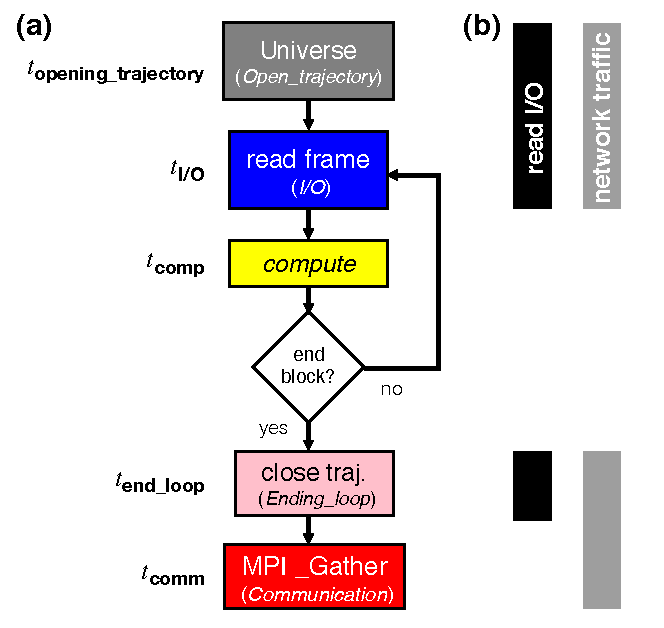
\includegraphics[width=7cm]{figures/flowchart.pdf}
  \caption{Flow chart of the MPI-parallelized RMSD algorithm, Algorithm~\ref{alg:RMSD}.
    \textbf{(a)} Each MPI process performs the same steps but reads trajectory frames from different blocks of the trajectory.
    The color scheme and labels in italics correspond to the colors and labels for measured timing quantities in the following graphs (e.g., Figs.~\protect\ref{fig:ScalingComputeIO} and \protect\ref{fig:MPIranks}).
    The names of the corresponding timing quantities from Table \protect\ref{tab:notation} are listed next to each step.
    \textbf{(b)} Steps that access the shared Lustre file system with read I/O are included in the black bars; steps that communicate via the shared InfiniBand network are included in the gray bars.
    The Lustre file system is accessed through the network and hence all I/O steps also use the network.
  }
  \label{fig:flowchart}
\end{figure}

As a test case that is representative of a common task in the analysis of biomolecular simulation trajectories we calculated the time series of the minimal structural root mean square distance  (\textbf{RMSD}) after rigid body superposition \cite{Lea96, Mura:2014kx}.
The RMSD is used to show the rigidity of protein domains and more generally characterizes structural changes.
It is calculated as a function of time $t$ as
\begin{equation}
  \label{eq:rmsd}
  \text{RMSD}(t) = \min_{\mathsf{R}, \mathbf{t}} %
  \sqrt{\frac{1}{N} \sum_{i=1}^{N} \left[ %
      (\mathsf{R}\cdot\mathbf{x}_{i}(t) + \mathbf{t}) - \mathbf{x}_{i}^{\text{ref}} \right]^{2}}
\end{equation}
where $\mathbf{x}_{i}(t)$ is the position of atom $i$ at time $t$, $\mathbf{x}_{i}^{\text{ref}}$ is its position in a reference structure and the distance between these two is minimized by finding the optimum $3\times3$ rotation matrix $\mathsf{R}$ and translation vector $\mathbf{t}$. 
The optimum rigid body superposition was calculated with the QCPROT algorithm~\cite{Liu:2010kx,Theobald:2005vn} (implemented in Cython and available through the \texttt{MDAnalysis.analysis.rms} module \cite{Gowers:2016aa}).

The RMSD trajectory analysis was parallelized as outlined in the flow chart in Figure~\ref{fig:flowchart}, with further details available in Algorithm~\ref{alg:RMSD}.
Each MPI process loads the core MDAnalysis structure (called the \texttt{Universe}), which includes loading a shared ``topology'' file with the simulation system information and opening the shared trajectory file.
Each process operates on a different block of frames and iterates through them by reading the coordinates of a single frame into memory and performing the RMSD computation with them.
Once all frames in the block are processed, the trajectory file is closed and results are communicated to MPI rank 0 using \texttt{MPI\_Gather()}.

The RMSD was determined for a subset of protein atoms, the $N=214$  C$_{\alpha}$ atoms of our test system (see section \ref{sec:data} for details).
The time complexity for the RMSD Algorithm~\ref{alg:RMSD} is $\mathcal{O}(T \times N^{2})$~\cite{Liu:2010kx} where $T$ is the number of frames in the trajectory and $N$ the number of particles included in the RMSD calculation.

\begin{algorithm}[ht!]
	\scriptsize
	\caption{MPI-parallel Multi-frame RMSD Algorithm}
	\label{alg:RMSD}
	\hspace*{\algorithmicindent} \textbf{Input:} \emph{size}: Total number of frames \\
	\hspace*{\algorithmicindent} \emph{ref}: mobile group in the initial frame which will be considered as reference \\
	\hspace*{\algorithmicindent} \emph{start \& stop}: Starting and stopping frame index\\
	\hspace*{\algorithmicindent} \emph{topology \& trajectory}: files to read the data structure from \\
	\hspace*{\algorithmicindent} \textbf{Output:} Calculated RMSD arrays
	\begin{algorithmic}[1]
		\Procedure{$Block\_RMSD$}{topology, trajectory, $ref$, start, stop}                       
		\State u $\leftarrow$ Universe(topology, trajectory)\Comment{u hold all the information of the physical system}
		\State $g$ $\leftarrow$ u.frames[start:stop]
		\For{$\forall iframe$ in $g$}
		\State $results[iframe] \leftarrow RMSD(g, ref)$
		\EndFor
		\State \Return results
		\EndProcedure
		\\        
		\State MPI Init
		\State rank $\leftarrow$ rank ID
		\State index $\leftarrow$ indices of mobile atom group
		\State xref0 $\leftarrow$ Reference atom group\textsc{\char13}s position
		\State out $\leftarrow$ Block\_RMSD(topology, trajectory, xref0, start=start, stop=stop)
		\\
		\State Gather(out, RMSD\_data, rank\_ID=0)
		\State MPI Finalize
	\end{algorithmic}
\end{algorithm}


\subsection{MPI for Python (\package{mpi4py})}
\label{sec:methods-mpi4py}

MPI for Python (\package{mpi4py}) is a Python wrapper for the Message Passing Interface (MPI) standard and allows any Python program to employ multiple processors \cite{Dalcin:2011aa, Dalcin:2005aa}.
Performance degradation due to using \package{mpi4py} is not prohibitive \cite{Dalcin:2011aa, Dalcin:2005aa} and the overhead is far smaller than the overhead associated with the use of interpreted versus compiled languages \cite{GAiN}.
Overheads in \package{mpi4py} are small compared to C code if efficient raw memory buffers are used for communication \cite{Dalcin:2011aa}, as used in the present study.

\subsection{Global Arrays Toolkit}
\label{sec:methods-ga}

The \package{Global Arrays} (GA) toolkit provides users with a language interface that allows them to distribute data while maintaining the type of global index space and programming syntax similar to what is available when programming on a single processor \cite{GA}.
\emph{Global Arrays} is implemented with Fortran-77 and C bindings and provides C++ and Python interfaces.
It allows manipulating physically distributed dense multi-dimensional arrays without explicitly defining communication and synchronization between processes.
The underlying communication is determined by a runtime environment, which defaults to the \emph{Communication runtime for Extreme Scale} (ComEx) \cite{Daily:2014aa}.
ComEx uses shared memory for intra-node communication and inter-node communication employs ComEx with MPI.
\emph{Global Arrays in NumPy} (GAiN) extends GA to Python through Numpy \cite{GAiN}. 
The \package{Global Arrays} toolkit provides functions to create global arrays (\texttt{ga\_create()}) and to copy data to (\texttt{ga\_put()}) and from (\texttt{ga\_get()}) such a global array,  as well as additional functions for copying between arrays and freeing them \cite{GAiN}.
When a global array is created (\texttt{ga\_create()}) each process will create an array of the same shape and size, physically located in the local memory space of that process \cite{GA}. 
The GA library maintains a list of all these memory locations, which can be queried with the \texttt{ga\_access()} function.
Using a pointer returned by \texttt{ga\_access()}, one can directly modify the data that is local to each process.
When a process tries to access a block of data the request is first decomposed into individual blocks representing the contribution to the total request from the data held locally on each process (\textit{B. J. Palmer and J. Daily, personal communication}).
The requesting process then makes individual requests to each of the remote processes. 

GA allows independent, asynchronous, and efficient access to logical blocks of physically distributed arrays, with no need for explicit cooperation by other processes; in particular, it allows data locality to be explicitly specified and used \cite{GA-NUMA}.
We investigated if communication cost could be reduced by using \package{Global Arrays}.
Algorithm \ref{alg:GA} describes the RMSD algorithm with \package{Global Arrays} instead of MPI.


\begin{algorithm}[ht!]
	\scriptsize
	\caption{MPI-parallel Multi-frame RMSD using Global Arrays}
	\label{alg:GA}
	\hspace*{\algorithmicindent} \textbf{Input:}\emph{size}: Total number of frames assigned to each rank $N_{b}$\\
	\hspace*{\algorithmicindent} \emph{g\_a}: Initialized Global Arrays \\
	\hspace*{\algorithmicindent} \emph{xref0}: mobile group in the initial frame which will be considered as reference \\
	\hspace*{\algorithmicindent} \emph{start \& stop}: that tell which block of trajectory (frames) is assigned to each rank \\
	\hspace*{\algorithmicindent} \emph{topology \& trajectory}: files to read the data structure from \\
	\hspace*{\algorithmicindent}\textbf{Include:} \texttt{Block\_RMSD()} from Algorithm \ref{alg:RMSD}
	\begin{algorithmic}[1]
		
		\State bsize $\leftarrow$ ceil(trajectory.number\_frames / size)
		\State g\_a $\leftarrow$ ga.create(ga.C\_DBL, [bsize*size,2], "RMSD")
		\State buf $\leftarrow$ np.zeros([bsize*size,2], dtype=float)
		\State out $\leftarrow$ Block\_RMSD(topology, trajectory, xref0, start=start, stop=stop)
		\State ga.put(g\_a, out, (start,0), (stop,2))
		\If{rank == 0}
		\State buf $\leftarrow$ ga.get(g\_a, lo=None, hi=None)
		\EndIf
	\end{algorithmic}
\end{algorithm}

\subsection{MPI and Parallel HDF5}
\label{sec:methods-hdf5}

HDF5 is a structured self-describing hierarchical data format which is the standard mechanism for storing large quantities of numerical data in Python (\url{http://www.hdfgroup.org/HDF5}, \cite{pythonhdf5}).
Parallel HDF5 (\package{PHDF5}) typically sits on top of a MPI-IO layer and can use MPI-IO optimizations. 
In \package{PHDF5}, all file access is coordinated by the MPI library; otherwise, multiple processes would compete over accessing the same file on disk. 
MPI-based applications launch multiple parallel instances of the Python interpreter that communicate with each other via the MPI library. 
Implementation is straightforward as long as the user supplies a MPI communicator and takes into account some constraints required for data consistency \cite{pythonhdf5}.
\package{HDF5} itself handles nearly all the details involved with coordinating file access when the shared file is opened through the \emph{mpio} driver.

MPI has two flavors of operation: collective (all processes have to participate in the same order) and independent (processes can perform the operation in any order or not at all) \cite{pythonhdf5}.
With \package{PHDF5}, modifications to file metadata must be performed collectively and although all processes perform the same task, they do not need to be synchronized \cite{pythonhdf5}. 
Other tasks and any type of data operations can be performed independently by processes.
In the present study, we use independent operations.

% -*- mode: latex; mode: visual-line; fill-column: 9999; coding: utf-8 -*-

\section{Benchmark Environment}
\label{sec:system}
Our benchmark environment consisted of three different XSEDE \cite{xsede} HPC resources (described in section~\ref{sec:hpcresources}), the software stack used (section~\ref{sec:software}), which had to be compiled for each resource, and the common test data set (section~\ref{sec:data}).

\subsection{HPC Resources}
\label{sec:hpcresources}

The computational experiments were executed on standard compute nodes of three XSEDE \cite{xsede} supercomputers, \emph{SDSC Comet}, \emph{PSC Bridges}, and \emph{LSU SuperMIC} (Table~\ref{tab:sys-config}).
\emph{SDSC Comet} is a 2 PFlop/s cluster with 2,020 compute nodes in total. It is optimized for running a large number of medium-size calculations (up to 1,024 cores) to support the most prevalent type of calculation on XSEDE resources.
\emph{PSC Bridges} is a 1.35 PFlop/s cluster with different types of computational nodes, including 16 GPU nodes, 8 large memory and 2 extreme memory nodes, and 752 regular nodes.
It was designed to flexibly support both traditional (medium scale calculations) and non-traditional (data analytics) HPC uses.
\emph{LSU SuperMIC} offers 360 standard compute nodes with a peak performance of 557 TFlop/s.
The parallel file system on all three machines is Lustre (\url{http://lustre.org/}) and is shared between the nodes of each cluster.

\begin{table}[ht!]
	\centering
	\begin{adjustbox}{max width=\textwidth}
		\begin{tabular}{c c c c c c c c c}
			\toprule
			\bfseries\thead{Name} & \bfseries\thead{Nodes} & \makecell{\bfseries\thead{Number \\of Nodes}} & \bfseries\thead{CPUs} &  \bfseries\thead{RAM} & \bfseries\thead{Network Topology} & \makecell{\bfseries\thead{Scheduler and  \\ Resource Manager}} & \makecell{\bfseries\thead{parallel\\file system}}\\
			\midrule
			\bfseries \emph{SDSC Comet} & Compute & 6400 & \makecell{2 Intel Xeon (E5-2680v3) \\ 12 cores/CPU, 2.5 GHz} &128 GB DDR4 DRAM & 56 Gbps IB & SLURM & Lustre\\
			\bfseries \emph{PSC Bridges} & RSM & 752 & \makecell{2 Intel Haswell (E5-2695 v3)  \\14 cores/CPU, 2.3 GHz} & 128 GB, DDR4-2133MHz & 12.37 Gbps OPA & SLURM & Lustre\\
			\bfseries \emph{LSU SuperMIC} & Standard & 360 & \makecell{2 Intel Ivy Bridge (E5-2680) \\10 cores/CPU, 2.8 GHz} & 64 GB, DDR3-1866MHz  & 56 Gbps IB & PBS & Lustre\\
			\bottomrule
		\end{tabular}
	\end{adjustbox}
	\caption[Configuration of HPC resources]
	{Configuration of the HPC resources that were benchmarked. Only a subset of the total available nodes were used. IB: InfiniBand; OPA: Omni-Path Architecture.}
	\label{tab:sys-config}
\end{table}

\subsection{Software}
\label{sec:software}

Table~\ref{tab:version} lists the tools and libraries that were required for our computational experiments.  Many domain specific packages are not available in the standard software installation on supercomputers.
We therefore had to compile them, which in some cases required substantial effort due to non-standard building and installation procedures or lack of good documentation.
Because this is a common problem that hinders reproducibility we provide detailed version information, notes on the installation process, as well as comments on the ease of installation and the quality of the documentation in Table~\ref{tab:version}.
For the MPI implementation we used Open MPI release 1.10.7  (\url{https://www.open-mpi.org/}) consistently everywhere.
Detailed instructions to create the computing environments together with the benchmarking code can be found in the GitHub repository.
Carefully setting up the same software stack on the three different supercomputers allowed us to clearly demonstrate the reproducibility of our results and showed that our findings were not dependent on machine specifics.


\begin{table}[ht!]
\centering
\begin{adjustbox}{max width=\textwidth}
\begin{tabular}{l c l c c l l}
  \toprule
            \bfseries\thead{Package} & \bfseries\thead{Version} & \bfseries\thead{Description} & \bfseries\thead{Ease of Installation} & \bfseries\thead{Documentation} & \bfseries\thead{Installation} & \bfseries\thead{Dependencies}\\
  \midrule
   \bfseries GCC & 4.9.4 & GNU Compiler Collection & 0 & ++ & \makecell[l]{via configuration \\files, environment \\or command line options, \\ minimal configuration \\ is required} &--\\
   \midrule
   \bfseries Open MPI & 1.10.7 & MPI Implementation & 0 & ++ & \makecell[l]{via configuration \\ files, environment \\or command line options, \\ minimal configuration \\ is required} &--\\
   \midrule
   \bfseries Global Arrays & 5.6.1 & Global Arrays & $-$ & + & \makecell[l]{via configuration files, \\ environment \\or command line options, \\ several optional configuration\\ settings available} & \makecell[l]{MAMA, ARMCI\\ MPI 1.x/2.x/3.x \\ implementation like \\ Open MPI \\ built with shared/dynamic\\ libraries, GCC}\\
   \midrule
   \bfseries Python & 2.7.13 & Python language & + & ++ & Conda Installation & --\\
   \midrule
   \bfseries MPI4py & 3.0.0 & MPI for Python & + & ++ & Conda Installation &\makecell[l]{Python 2.7 or above, \\ MPI 1.x/2.x/3.x  \\ implementation like \\ Open MPI \\built with shared/dynamic \\libraries, Cython}\\
   \midrule
   \bfseries GA4py & 1.0 & Global Arrays for Python & 0 & 0 & Python setuptools &\makecell[l]{Global Arrays, Python 2 only,\\ MPI 1.x/2.x/3.x  \\implementation like \\ Open MPI \\ built with shared/dynamic \\libraries, Cython,  \\MPI4py, Numpy} \\
   \midrule
   \bfseries PHDF5 & 1.10.1 & Parallel HDF5 & $-$ & ++ & \makecell[l]{via configuration files,\\ environment \\or command line options, \\ several optional configuration\\ settings available} &\makecell[l]{MPI 1.x/2.x/3.x  \\ implementation like \\ Open MPI  \\GNU, MPIF90,  \\MPICC, MPICXX}\\
   \midrule
   \bfseries H5py &  2.7.1 & Pythonic wrapper around the HDF5 & + & ++ & Conda Installation & \makecell[l]{Python 2.7, or above,\\ PHDF5, Cython}\\    
   \midrule
   \bfseries MDAnalysis & 0.17.0 & \makecell[l]{Python library to analyze \\trajectories from MD simulations} & + & ++ & Conda Installation & \makecell[l]{Python $>=$2.7, Cython,\\ GNU, Numpy}\\
  \bottomrule
\end{tabular}
\end{adjustbox}
\caption[Version of the packages used in the present study]%
{Detailed comparison on the dependencies and installation of different software packages used in the present study. Software was built from source or obtained via a package manager and installed on the multi-user HPC systems in Table~\protect\ref{tab:sys-config}. Evaluation of ease of installation and documentation uses a subjective scale with ``++'' (excellent), ``+'' (good), ``0'' (average), and ``$-$'' (difficult/lacking) and reflects the experience of a typical domain scientist at the graduate/post-graduate level in a discipline such as computational biophysics or chemistry.}
\label{tab:version}
\end{table}


\subsection{Data Set}
\label{sec:data}

The test system contained the protein adenylate kinase with 214 amino acid residues and 3341 atoms in total~\cite{Seyler:2014il} and the topology information (atoms types and bonds) was stored in a file in CHARMM PSF format.
The test trajectory was created by concatenating 600 copies of a MD trajectory with 4,187 time frames (saved every 240~ps for a total simulated time of 1.004~$\mu\text{s}$) in CHARMM DCD format~\cite{Seyler:2017aa} and converting to Gromacs XTC format trajectory, as described for the ``600x'' trajectory in~\citet{Khoshlessan:2017ab}.
The trajectory had a file size of about 30 GB and contained 2,512,200 frames (corresponding to 602.4~$\mu\text{s}$ simulated time).
The file size was relatively small because water molecules that were also part of the original MD simulations were stripped to reduce the original file size by a factor of about 10; such preprocessing is a common approach if one is only interested in the protein behavior.
Thus, the trajectory represents a small to medium system size in the number of atoms and coordinates that have to be loaded into memory for each time frame.
The XTC format is a format with lossy compression \cite{Lindahl01, Spangberg:2011zr}, which also contributed to the compact file size.
XTC trades lower I/O demands for higher CPU demands during decompression and therefore performed well in our previous study~\cite{Khoshlessan:2017ab}.
Although 2,512,200 frames represents a long simulation for current standards, such trajectories will become increasingly common due to the use of special hardware~\cite{Shaw:2009ly, Shaw:2014aa} and GPU-acceleration~\cite{Salomon-Ferrer:2013cr, Glaser:2015ys, Abraham:2015aa}.

\label{methods}

\subsection{Timing observables}
We model MPI performance based on the RMSD algorithm (\ref{alg:RMSD}) and Dihedral Featurization algorithm (\ref{alg:Dihedral}). 
The notation for our models is summarized in Table \ref{tab:notation}.
Inside the code, relevant probs were taken and stored. 
We will abbreviate the timings in the following as variables $t_{Ln}$ where $Ln$ refers to the line number in algorithm \ref{alg:RMSD}.
Similar calculations can be used for all other algorithms.

We directly measured inside our code (in the function \texttt{block\_rmsd()}) the ``I/O'' time for
ingesting the data from the file system into memory, ($t_{I/O}^{frame} = t_{L4}$) and the ``compute'' time per
trajectory frame to perform the computation ($t_{comp}^{frame} = t_{L5}$). 
 \tIO is the summation of ``I/O'' time per frame and \tcomp is the summation of ``compute'' time per frame for all the frames assigned to each rank ($N_{frames}$). 
$t_{end\_loop} = t_{L6}+t_{L7}$ is the time delay between the end of the last iteration and exiting the for loop.
$t_{opening\_trajectory} = t_{L2}+t_{L3}$ is the time which data structures are initialized and topology and trajectory files are opened (problem setup).

$t_{Communication_{MPI}} = t_{L16}$ is the time ``Shuffle'' time to gather (``reduce'') all data from all processor ranks to rank zero.
The total time (for all frames) spent in \texttt{block\_rmsd()} is $t_{\text{RMSD}} = t_{L1} + ...+ t_{L8}$. 
There are parts of the code in \texttt{block\_rmsd()} that are not covered by the detailed timing information of \tcomp and \tIO. 
To measure the un-accounted time we define the ``overheads''.
$t_{Overhead1}$ and $t_{Overhead2}$ are the overhead of the calculations and they should be ideally very small.  
The total time to completion for a single process on $N$ cores is $t_{N}$, which is mathematically equivalent to
$t_{N} \equiv t_{RMSD} + \tcomm$.

\subsection{Performance Measurement}
We also recorded the total time to solution $t_{\text{total}}(N)$ with $N$ MPI processes on $N$ cores (which is effectively
$t_{\text{total}}(N) \approx \max t_{N}$). 
Strong scaling was quantified by calculating the speed-up relative to performance on a single core and efficiency (using MPI).

\begin{gather}
  \label{eq:speedup}
  S = \frac{t_{\text{total}}(N)}{t_{\text{total}}(1)}
\end{gather}

\begin{gather}
  \label{eq:efficiency}
  E = \frac{S}{N}
\end{gather}

Additionally, we introduce two important performance parameters that determines whether we observe stragglers.
We define this parameter as the ratio of compute time to I/O time:

\begin{gather}
  \label{eq:Compute-I/O}
    \frac{\bar{t}_{comp}^{frame}}{\bar{t}_{IO}^{frame}} \approx \frac{\tcomp}{\tIO} 
 \end{gather}

and the ratio of compute to communication time\mknote{This equation should be corrected}:

\begin{gather}
  \label{eq:Compute-comm}
    \frac{\bar{t}_{comp}}{\bar{t}_{communication}} \approx \frac{\tcomp}{\tcomm} 
 \end{gather}
 
\begin{table}[ht!]
\centering
\begin{tabular}{c c}
  \toprule
           \bfseries\thead{Item} & \bfseries\thead{Definition}\\
  \midrule
    $N_{frames}$ & $N_{frames}^{total}/N$\\  
    $t_{end\_loop}$ & $t_{L6}+t_{L7}$\\
    $t_{opening\_trajectory}$ &  $t_{L2}+t_{L3}$ \\
    $t_{comp}$ & $\sum_{1}^{N_{frames}}t_{comp}^{frame}$\\
    $t_{IO}$ & $\sum_{1}^{N_{frames}}t_{I/O}^{frame}$\\
    $t_{all\_frame}$ & $t_{L4}+t_{L5}+t_{L6}$  \\
    $t_{RMSD}$ &  $t_{L1} + ...+ t_{L8}$ \\
    $t_{Communication_{MPI}}$ &  $t_{L16}$  \\
    $t_{Communication_{GA}}$ &  $t_{L5}+t_{L6}+t_{L7}+t_{L8}$  \\
    $t_{Overhead1}$ & $t_{all\_frame}-t_{IO\_final}-t_{comp\_final}-t_{end\_loop}$  \\
    $t_{Overhead2}$ & $t_{RMSD}-t_{all\_frame}-t_{opening\_trajectory}$  \\
    $t_{N}$ & $t_{RMSD}+t_{Communication}$ \\
    $t_{total}$ & $\max t_{N}$ \\
  \bottomrule
\end{tabular}
\caption[Summary of the notation of our performance modeling]
{Summary of the notation of our performance modeling. Relevant probes in the codes are taken and stored,
which we will abbreviate in here as $t_{Ln}$ where {Ln} refers to the line number in the corresponding algorithm. 
$t_{Communication_{MPI}}$ and $t_{Communication_{GA}}$ are both referred to $t_{Communication}$ in the text}
\label{tab:notation}
\end{table}


\label{impl_exp}

\subsection{RMSD Benchmark}
\label{sec:RMSD}
The RMSD algorithm represents a task whose computational load is smaller than the I/O load per frame (typical values $t_{\text{compute}}^{\text{frame}} = 0.09\ \text{ms}$, $t_{\text{IO}}^{\text{frame}} = 0.3\ \text{ms}$, thus $\overline{\tcomp}/\overline{\tIO} \approx 0.3$). 
We showed in~\cite{Khoshlessan:2017ab} that the RMSD task only scaled well up \gpnote{I removed the number of cores because Stampede had 16 cores and Comet has 24}on a single compute node on \emph{SDSC Comet}, and \emph{TACC Stampede}, using either Dask or MPI.

We focus on the MPI implementation (via \package{mpi4py}~\cite{Dalcin:2011aa, Dalcin:2005aa}) to better understand the cause for the lack of scaling across nodes.
As in our previous work, we also observed very poor strong scaling performance (Figures~\ref{fig:MPIscaling},~\ref{fig:MPIspeedup} and~\ref{fig:MPIscaling-Bridges} and~\ref{fig:MPIspeedup-Bridges}) beyond a single node.
A more detailed analysis showed that the RMSD computation, and to a lesser degree the I/O, considered on their own scaled well beyond 50 cores (yellow and blue lines in Figure~\ref{fig:ScalingComputeIO}). 
But, communication (red line in Figure~\ref{fig:ScalingComputeIO}) and the initial file opening (gray line in Figure~\ref{fig:ScalingComputeIO}) started to dominate beyond 50 cores.
Communication cost and initial time for opening the trajectory were distributed unevenly across MPI ranks, as shown in Figure~\ref{fig:MPIranks}. 
The ranks that took much longer to complete than the typical execution time of the other ranks were the stragglers that hurt performance.

\subsubsection*{Identification of Scalability Bottlenecks}
In the example shown in Figure~\ref{fig:MPIranks}, 62 ranks out of 72 took about $60sec$ (the stragglers) whereas the remaining ranks only took about $20sec$. 
The detailed breakdown of the time spent on each rank (Figure~\ref{fig:MPIranks}) showed that the computation, \tcomp, was relatively constant across ranks. 
The time spent on reading data from the shared trajectory file on Lustre into memory, \tIO, showed variability across different ranks. 
The stragglers, however, appeared to be defined by occasionally much larger \emph{communication} times, \tcomm (line 16 in Algorithm~\ref{alg:RMSD}), which were on the order of $30sec$, and by larger times to initially open the trajectory (line 2 in Algorithm~\ref{alg:RMSD}).
\tcomm varied across different ranks and was barely measurable for a few of them.
Although the data in Figure~\ref{fig:MPIranks} represent one run and in other instances different number of ranks were stragglers, the overall hypothesis was confirmed by the averages over five independent repeats and all ranks (Figure~\ref{fig:ScalingComputeIO}).
This initial analysis indicated that communication was a major issue that prevented good scaling beyond a single node but the problems related to file I/O also played an important role in limiting performance.

\begin{figure}
\centering
\begin{subfigure}{.4\textwidth}
  \includegraphics[width=\linewidth]{figures/main-RMSD-t_total.pdf}
  \captionsetup{format=hang}
  \caption{Scaling total (five repeats)}
  \label{fig:MPIscaling}
\end{subfigure}
\hfill
\begin{subfigure}{.4\textwidth}
  \includegraphics[width=\linewidth]{figures/main-RMSD-speed_up.pdf}
  \captionsetup{format=hang}
  \caption{Speed-up (five repeats)}
  \label{fig:MPIspeedup}
\end{subfigure}
\bigskip

\begin{subfigure}{.4\textwidth}
  \includegraphics[width=\linewidth]{figures/main-RMSD-time_comp_IO_comparison.pdf}
  \captionsetup{format=hang}
\caption{Scaling for different components (five repeats)}
\label{fig:ScalingComputeIO}
\end{subfigure}
\hfill
\begin{subfigure} {.5\textwidth}
  \includegraphics[width=\linewidth]{figures/main-RMSD-BarPlot-rank-comparison_72_5.pdf}
  \captionsetup{format=hang}
  \caption{Time comparison on different parts of the calculations per MPI rank (example)}
  \label{fig:MPIranks}
\end{subfigure}

\caption{Performance of the RMSD task (I/O-bound with $\overline{\tcomp}/\overline{\tIO} \approx 0.3$) with MPI on \emph{SDSC Comet}.
Results were communicated back to rank 0. Five independent repeats were performed to collect statistics. (a-c) The error bars show
standard deviation with respect to mean. (d) Compute \tcomp, IO \tIO, communication \tcomm, ending the for loop $t_{\text{end\_loop}}$,
  opening the trajectory $t_{\text{opening\_trajectory}}$, and overheads $t_{\text{overhead1}}$, $t_{\text{overhead2}}$ per MPI rank (see Table \ref{tab:notation} for the definition).
These are data from one run of the five repeats. MPI ranks 0, 12--27 and 29--72 are stragglers. \textbf{Note:} In serial, there is no communication.}
\label{fig:MPIwithIO}
\end{figure} 

\subsubsection*{Influence of Hardware}
We ran the same benchmarks on multiple HPC systems (XSEDE's \emph{PSC Bridges} (Fig.~\ref{fig:MPIwithIO-Bridges}) and \emph{LSU SuperMIC} (Fig.~\ref{fig:MPIwithIO-SuperMIC})), and observed the occurrence of stragglers, in a manner very similar to the results described for \emph{SDSC Comet}.
There was no clear pattern in which certain MPI ranks would always be a straggler, neither could we trace stragglers to specific cores or nodes.
Therefore, the phenomenon of stragglers in the RMSD case was reproducible on different clusters and thus appeared to be independent from the underlying hardware.

\subsection{Effect of average compute over average IO ratio on Performance}
\label{sec:bound}

The results in section~\ref{sec:RMSD} indicated communication and I/O to be two important factors that appeared to correlate with stragglers. 
In order to better characterize the RMSD task, we computed the ratio between the time to complete the computation and the time spent on I/O, $\overline{\tcomp}/\overline{\tIO} = 0.3$, and found that this task was I/O bound, i.e.,
\begin{gather*}
  \frac{\overline{\tcomp}}{\overline{\tIO}} \ll 1.
\end{gather*}

For such a I/O-bound task we were not able to achieve good scaling beyond a single node. 
We hypothesized that decreasing the relative I/O load with respect to the compute load would also reduce the impact of stragglers by interleaving I/O with longer periods of computation and thus reducing the impact of I/O contention.
We therefore set out to measure compute bound tasks, i.e.\ ones with
\begin{gather*}
  \frac{\overline{\tcomp}}{\overline{\tIO}} \gg 1.
\end{gather*}
To measure the effect of the $\overline{\tcomp}/\overline{\tIO}$ ratio on performance but leaving other parameters the same, we artificially increased the computational load by repeating the same RMSD calculation (line 10, algorithm \ref{alg:RMSD}) 40, 70 and 100 times in a loop, resulting in forty-fold (``$40\times$''), seventy-fold (``$70\times$''), and one hundred-fold (``$100\times$'') load increases.

\subsubsection{Effect of Increased Compute workload for RMSD Task}

The increased computational workloads corresponded to $\overline{\tcomp}/\overline{\tIO}$ ratios of 11, 19, 27 respectively as shown in Table \ref{tab:load-ratio}.
\gpnote{I am not sure if this breaking passes the same message. It needs fixing.}
In fact, the $\overline{\tcomp}/\overline{\tIO}$ ratio for the higher workloads (with factor $X$) should be $X$ times the $\overline{\tcomp}/\overline{\tIO}$ for the $1\times$ workload (in agreement with theoretical prediction in Table \ref{tab:load-ratio}).
This is since on average the I/O workload of each rank is $N_{\text{b}} \times \tIO $, which is independent of $X$. 
However, the workload for the computation is $X \times N_{\text{b}} \times \tcomp$, and hence the ratio is $X \times \overline{\tcomp}/\overline{\tIO}$.

\begin{table}[ht!]
\centering
\begin{tabular}{rrrrr}
  \toprule
  \bfseries\thead{Workload} &  \bfseries\thead{$\tcomp$} &  \bfseries\thead{$\tIO$}
  & \multicolumn{2}{c}{\bfseries\thead{$\overline{\tcomp}/\overline{\tIO}$}}\\
  & & & \thead{measured} & \thead{theoretical}\\
  \midrule
    $1\times$   &   226 & 791 &  0.29 &   \\  
    $40\times$  &  8655 & 791 & 11   & 11\\    
    $70\times$  & 15148 & 791 & 19   & 20\\  
    $100\times$ & 21639 & 791 & 27   & 29\\  
  \bottomrule
\end{tabular}
\caption[Change in load-ratio with RMSD workload]{Change in $\overline{\tcomp}/\overline{\tIO}$ ratio with change in the RMSD workload.
  The RMSD workload was artificially increased in order to examine the effect of compute to I/O ratio on the performance.
  The reported compute and I/O time were calculated based on the serial version using one core and used to calculate the measured $\overline{\tcomp}/\overline{\tIO}$.
  The theoretical $\overline{\tcomp}/\overline{\tIO}$ (see text) is provided for comparison.}
\label{tab:load-ratio}
\end{table}

We performed this experiment to show the effect of the $\overline{\tcomp}/\overline{\tIO}$ ratio on performance (Figure~\ref{fig:tcomp_tIO_effect}).
As the $\overline{\tcomp}/\overline{\tIO}$ ratio increased, speed-up and performance improved, and showed overall better scaling than the I/O-bound workload, i.e. $1\times$ RMSD (Figure~\ref{fig:S1_tcomp_tIO_effect}).
The RMSD calculation consistently scaled up to larger numbers of cores ($N=56$ for $70\times$ RMSD) for higher $\overline{\tcomp}/\overline{\tIO}$ ratios.
Figures \ref{fig:S2_tcomp_tIO_effect} and \ref{fig:E_tcomp_tIO_effect} show that speed-up and efficiency approach their ideal value for each processor count with increasing $\overline{\tcomp}/\overline{\tIO}$ ratio.

\begin{figure}[ht!]
\centering
\begin{subfigure} {.3\textwidth}
  \includegraphics[width=\linewidth]{figures/Compute_to_IO_ratio_on_performance_2d_v17.pdf}
  \caption{Speed-Up}
  \label{fig:S1_tcomp_tIO_effect}
\end{subfigure}
\hfill
\begin{subfigure}{.3\textwidth}
  \includegraphics[width=\linewidth]{figures/Compute_to_IO_ratio_on_performance_2d_2_v17.pdf}
  \caption{Speed-Up}
  \label{fig:S2_tcomp_tIO_effect}
\end{subfigure}
\hfill
\begin{subfigure}{.3\textwidth}
  \includegraphics[width=\linewidth]{figures/Compute_to_IO_ratio_on_performance_2d_3_v17.pdf}
  \caption{Efficiency}
  \label{fig:E_tcomp_tIO_effect}
\end{subfigure}
%
\caption{Effect of $\overline{\tcomp}/\overline{\tIO}$ ratio on performance of the RMSD task with MPI performed on \emph{SDSC Comet}. We tested performance for $\overline{\tcomp}/\overline{\tIO}$ ratios of 0.3, 11, 19, 27.
which correspond to $1\times$ RMSD, $40\times$ RMSD, $70\times$ RMSD, and $100\times$ RMSD respectively. (a) Effect of $\overline{\tcomp}/\overline{\tIO}$ on the Speed-Up
(b) Change in the Speed-Up with respect to $\overline{\tcomp}/\overline{\tIO}$ for different processor counts (c) Change in the efficiency with respect to $\overline{\tcomp}/\overline{\tIO}$ for different processor counts}
\label{fig:tcomp_tIO_effect}
\end{figure}

Even for moderately compute-bound workloads, such as the $40\times$ and $70\times$ RMSD tasks, increasing the computational workload over I/O reduced the impact of stragglers. Although, they still contributed to large variations in timing across different ranks and thus irregular scaling.

\subsubsection{I/O leads to stragglers}

In order to study an extreme case of a compute-bound task, we eliminated all I/O from the RMSD task by generating artificial trajectory data randomly in memory.
Without any I/O, performance improved markedly (Figure~\ref{fig:MPIwithoutIO}), with reasonable scaling up to 72 cores (3 nodes).
No stragglers were observed although an increase in communication time prevented ideal scaling performance.
Although in practice I/O cannot be avoided, this experiment demonstrated that accessing the trajectory file on the Lustre file system is at least one cause for the observed stragglers.

\subsection{Reducing Communication Cost: Application of Global Arrays}
\label{Global-Array}
As seen in Figure~\ref{fig:MPIranks} for small $\overline{\tcomp}/\overline{\tIO}$, communication acted as a scalability bottleneck. 
When the processes communicated result arrays back to the master process (rank 0), some processes took much longer as compared to others.
We therefore investigated strategies to reduce communication cost. 

We used Global Arrays (GA)~\cite{GA, GAiN} instead of collective communication in MPI and examined the change in the performance. 
In GA, we define one large RMSD array called \emph{global array}, and each MPI rank updates its associated block in the global RMSD array using \texttt{ga\_put()}. 
At the end, when all the processes exit \texttt{block\_rmsd()} function and update their local block in the global array, rank 0 will access the whole global array using \texttt{ga\_access()}.
In GA, the time for communication is $t_{\text{ga\_put()}}+t_{\text{ga\_access()}}$. 

Using Global Arrays improved the strong scaling performance (Figures~\ref{fig:MPIscaling-ga4py} and~\ref{fig:MPIspeedup-ga4py}) by reducing the communication time.
Nevertheless, the remaining variation in the trajectory I/O part of the calculation and in particular the initial opening of the trajectory prevented ideal scaling (Figure~\ref{fig:ScalingComputeIO-ga4py}).
Figure~\ref{fig:MPIranks-ga4py} shows that stragglers were primarily due to the fact that all ranks had to open the same trajectory file at the beginning of the execution.
In this case, these slow processes took about $50sec$, which was slower than the mean execution time of all other ranks of $17sec$. 
Trajectory opening was already problematic in the initial test (Figure~\ref{fig:ScalingComputeIO}), which was still dominated by the communication cost. By substantially reducing communication cost, the simultaneous trajectory opening by multiple ranks emerged as the next dominant cause for stragglers.
The improvement in performance can be attributed to the mitigation in the interference of MPI traffic with IO traffic as also studied in~\cite{Brown:2018ab}.

\begin{figure}[ht!]
\centering
\begin{subfigure}{.4\textwidth}
  \includegraphics[width=\linewidth]{figures/RMSD-ga4py-t_total.pdf}
  \captionsetup{format=hang}
  \caption{Scaling total}
  \label{fig:MPIscaling-ga4py}
\end{subfigure}
\hfill
\begin{subfigure}{.4\textwidth}
  \includegraphics[width=\linewidth]{figures/RMSD-ga4py-speed_up.pdf}
  \captionsetup{format=hang}
  \caption{Speed-up}
  \label{fig:MPIspeedup-ga4py}
\end{subfigure}
\bigskip

\begin{subfigure}{.4\textwidth}
  \includegraphics[width=\linewidth]{figures/RMSD-ga4py-time_IO_comparison.pdf}
  \captionsetup{format=hang}
\caption{Scaling for different components}
\label{fig:ScalingComputeIO-ga4py}
\end{subfigure}
\hfill
\begin{subfigure} {.5\textwidth}
  \includegraphics[width=\linewidth]{figures/RMSD-ga4py-BarPlot-rank-comparison_72_1.pdf}
  \captionsetup{format=hang}
  \caption{Time comparison on different parts of the calculations per MPI rank}
  \label{fig:MPIranks-ga4py}
\end{subfigure}

\caption{Performance of the RMSD task with MPI using Global Arrays ($\overline{\tcomp}/\overline{\tIO} \approx 0.3$) on SDSC Comet.
All ranks update the Global Arrays (\texttt{ga\_put()}) and rank 0 accesses the whole RMSD array through the global memory address (\texttt{ga\_get()}).
Five repeats were performed to collect statistics. (a-c) The error bars show standard deviation with respect to mean. 
(d) Compute \tcomp, IO \tIO, communication \tcomm, access to the whole Global Arrays by rank 0, $t_{\text{Access\_Global\_Array}}$, ending the for loop $t_{\text{end\_loop}}$,
  opening the trajectory $t_{\text{opening\_trajectory}}$, and overheads $t_{\text{overhead1}}$, $t_{\text{overhead2}}$ per MPI rank (See Table \ref{tab:notation} for the definition). 
  This is typical data from one run of the 5 repeats. MPI ranks 20 and 56 are stragglers, i.e., 
their total time far exceeds the mean of the all ranks. \textbf{Note:} In serial, there is no communication.}
\label{fig:MPIwithIO-ga4py}
\end{figure}

Motivated by the results in this section, we investigated the influence of the ratio of compute to communication costs ($\overline{\tcomp}/\overline{\tcomm}$) on performance in \ref{sec:tcomm}.
We found evidence to support the hypothesis that a larger ratio was beneficial, provided I/O costs could also be reduced, as discussed in the next section.

\subsection{Reducing I/O Cost}
\label{sec:I/O}
In order to improve performance we needed to employ strategies to avoid the competition over file access across different ranks when the $\overline{\tcomp}/\overline{\tIO}$ ratio was small.
To this end, we experimented with two different ways for reducing the I/O cost:
\begin{inparaenum}[1)]
	\item splitting the trajectory file into as many segments as the number of processes, thus using file-per-process access, and
	\item using the HDF5 file format together with MPI-IO parallel reads instead of the XTC trajectory format.
\end{inparaenum}
We discuss these two approaches and their performance improvements in detail in the following sections.

\subsubsection{Splitting the Trajectories (``subfiling'')}
\label{splitting-traj}
Subfiling is a mechanism previously used for splitting a large multi-dimensional global array to a number of smaller subarrays in which each smaller array is saved in a separate file. Subfiling reduces the file system control overhead by decreasing the number of processes concurrently accessing a shared file~\cite{scalable-IO, scalable-IO1}.
Because subfiling is known to improve programming flexibility and performance of parallel shared-file I/O, we investigated splitting our trajectory file into as many trajectory segments as the number of processes.
The trajectory file was split into $N$ segments, one for each process, with each segment having $N_{b}$ frames. 
This way, each process would access its own trajectory segment file without competing for file accesses. 

\paragraph{Performance with MPI communication}
We ran a benchmark up to 8 nodes (192 cores) and observed rather better scaling behavior with efficiencies above 0.6 (Figure~\ref{fig:MPIscaling-split} and~\ref{fig:MPIspeedup-split}) with the delay time for stragglers reduced from $65sec$ to about $10sec$ for 72 processes. 
However, scaling is still far from ideal due to communication (using MPI). 
Although the delay due to communication was much smaller as compared to parallel RMSD with shared-file I/O (compare Figure~\ref{fig:MPIranks-split} ($\tcomm^{\text{Straggler}} \gg \tcomp+\tIO$) to Figure~\ref{fig:MPIranks} ($\tcomm^{\text{Straggler}} \approx \tcomp+\tIO$)), it is still delaying several processes and resulted in longer job completion times (Figure~\ref{fig:MPIranks-split}). 
These delayed tasks impacted performance so that speed-up remained far from ideal (Figure~\ref{fig:MPIspeedup-split}).

\begin{figure}[ht!]
\centering
\begin{subfigure}{.32\textwidth}
  \includegraphics[width=\linewidth]{figures/Comparison_IO_compute_scaling_traj_splitting.pdf}
  \captionsetup{format=hang}
  \caption{Scaling for different components}
  \label{fig:ScalingComputeIO-split}
\end{subfigure}
\hfill
\begin{subfigure}{.3\textwidth}
  \includegraphics[width=\linewidth]{figures/Comparison_tot_time_traj_splitting.pdf}
  \caption{Scaling total}
  \label{fig:MPIscaling-split}
\end{subfigure}
\hfill
\begin{subfigure}{.3\textwidth}
  \includegraphics[width=\linewidth]{figures/Comparison_Speed_UP_traj_splitting.pdf}
  \captionsetup{format=hang}
  \caption{Speed-up}
  \label{fig:MPIspeedup-split}
\end{subfigure}
\bigskip

\begin{subfigure} {.45\textwidth}
  \includegraphics[width=\linewidth]{figures/split-BarPlot-rank-comparison_192_5.pdf}
  \captionsetup{format=hang}
   \caption{Time comparison on different parts of the calculations per MPI rank without Global Arrays}
  \label{fig:MPIranks-split}
\end{subfigure}
\hfill
\begin{subfigure} {.5\textwidth}
  \includegraphics[width=\linewidth]{figures/split-ga-BarPlot-rank-comparison_192_5.pdf}
  \captionsetup{format=hang}
  \caption{Time comparison on different parts of the calculations per MPI rank using Global Arrays}
  \label{fig:MPIranks-split-ga}
\end{subfigure}

\caption{Comparison on the performance of the RMSD task ($\overline{\tcomp}/\overline{\tIO} \approx 0.3$) on \emph{SDSC Comet} when the trajectories are split. For communicating the results, either Global Arrays (``ga'') or MPI (no Global Arrays, ``No-ga'') was used.  In the case of Global Arrays, all ranks updates the Global Arrays (\texttt{ga\_put()}) and rank 0 accessed the whole RMSD array through the global memory address (\texttt{ga\_get()}).  Five repeats were performed to collect statistics. (a) Compute and I/O scaling versus number of processes (b) Total time scaling versus number of processes (c) Speed-up (a-c) The error bars show standard deviation with respect to mean. (d-e) Compute \tcomp, IO \tIO, communication \tcomm, access to the whole Global Arrays by rank 0, $t_{\text{Access\_Global\_Array}}$, ending the for loop $t_{\text{end\_loop}}$, opening the trajectory $t_{\text{opening\_trajectory}}$, and overheads $t_{\text{overhead1}}$, $t_{\text{overhead2}}$ per MPI rank (see Table \ref{tab:notation} for the definitions). When Global Arrays was not used, the performance was decreased due to the non-uniform communication time across different ranks. However, with Global Arrays communication time was significantly reduced and scaling was close to ideal. \textbf{Note:} In serial, there is no communication.}
\label{fig:MPIwithIO-split}
\end{figure}

\paragraph{Performance using Global Arrays}
In Section~\ref{Global-Array} we showed that Global Arrays substantially reduced the communication cost. 
We wanted to quantify the performance when splitting the trajectory file while using Global Arrays.
Under otherwise identical conditions as in the previous section we now observed near ideal scaling behavior with efficiencies above 0.9 (Figure~\ref{fig:MPIscaling-split} and~\ref{fig:MPIspeedup-split}) without any straggler tasks (Figure~\ref{fig:MPIranks-split-ga}).
Although the reason why in our case Global Arrays appeared to be more efficient than direct MPI-based communication remains unclear, these results showed that contention for file access clearly impacted performance. By removing the contention, near ideal scaling could be achieved.

\paragraph{Further considerations for splitting trajectories}
The subfiling approach appears promising but it requires preprocessing of trajectory files and additional storage space for the segments.
We benchmarked the necessary time for splitting the trajectory using different number of MPI processes (Table~\ref{tab:timing-splitting}).
These preprocessing times were not included in the estimates because we are focusing on better understanding the principle causes of stragglers and we wanted to make the results directly comparable to the results of the previous sections.
Nevertheless, from an end user perspective, preprocessing of trajectories can be integrated in workflows (especially as the data in Table~\ref{tab:timing-splitting} indicate good scaling) and the preprocessing time can be quickly amortized if the trajectories are analyzed repeatedly.

Often trajectories from MD simulations on HPC machines are produced and kept in small chunks that would need to be concatenated to form a trajectory but that might be useful for the subfiling approach.
However, it might not be feasible to have exactly one trajectory segment per MPI rank.
In~\ref{sec:chainreader} we investigated if existing functionality in MDAnalysis that can create virtual trajectories from trajectory segments could benefit from the subfiling approach.
We found some improvements in performance but discovered limitations in the design that first have to be overcome before equivalent performance can be reached.
 
\subsubsection{MPI-based Parallel HDF5}
\label{HDF5}
Another approach we examined to improve I/O scaling was MPI-based Parallel HDF5. 
We converted our XTC trajectory file into a simple custom HDF5 format so that we could test the performance of parallel I/O with the HDF5 file format.
The code for this file format conversion can be found in the GitHub repository.
The time it took to convert our XTC file with $2,512,200$ frames into HDF5 format was about $5,400sec$ on a local workstation with network file system (NFS).

We ran our benchmark on up to 16 nodes (384 cores) and we observed near ideal scaling behavior with parallel efficiencies above 0.8 up to 8 nodes (Figure~\ref{fig:comparison_efficiency} and Figures~\ref{fig:MPIscaling-hdf5} and~\ref{fig:MPIspeedup-hdf5}) with no straggler tasks (Figure~\ref{fig:MPIranks-hdf5}).
The trajectory reading I/O (\tIO) was the dominant contribution, followed by compute (\tcomp), but because both contributions scaled well, overall scaling performance remained good, even for 384 cores.
We observed a low-performing outlier for 12 nodes (288 cores) with slower I/O than typical but did not further investigate.
Importantly, the trajectory opening cost remained negligible (in the millisecond range) and the cost for MPI communication also remained small (below 0.1 s, even for 16 nodes).
Overall, parallel MPI with HDF5 appears to be a robust approach to obtain good scaling, even for I/O-bound tasks.

\begin{figure}[ht!]
\centering
\begin{subfigure}{.4\textwidth}
  \includegraphics[width=\linewidth]{figures/hdf5-t_total.pdf}
  \caption{Scaling total}
  \label{fig:MPIscaling-hdf5}
\end{subfigure}
\hfill
\begin{subfigure}{.4\textwidth}
  \includegraphics[width=\linewidth]{figures/hdf5-speed_up.pdf}
  \caption{Speed-up}
  \label{fig:MPIspeedup-hdf5}
\end{subfigure}
\bigskip

\begin{subfigure}{.4\textwidth}
\centering
  \includegraphics[width=\linewidth]{figures/hdf5-time_comp_IO_comparison.pdf}
  \captionsetup{format=hang}
\caption{Scaling for different components}
\label{fig:ScalingComputeIO-hdf5}
\end{subfigure}
\hfill
\begin{subfigure} {.5\textwidth}
  \includegraphics[width=\linewidth]{figures/hdf5-BarPlot-rank-comparison_192_4.pdf}
  \captionsetup{format=hang}
  \caption{Time comparison on different parts of the calculations per MPI rank}
  \label{fig:MPIranks-hdf5}
\end{subfigure}
%
\caption{Performance of the RMSD task with MPI-based parallel HDF5 ($\overline{\tcomp}/\overline{\tIO} \approx 0.3$) on SDSC Comet.
Data are read from the file system from a shared HDF5 file format instead of XTC format (Independent I/O) and results are communicated back to rank 0 (communications included). 
Five repeats were performed to collect statistics. (a-c) The error bars show standard deviation with respect to mean. (d) Compute \tcomp, IO \tIO, communication \tcomm, ending the for loop $t_{\text{end\_loop}}$,
  opening the trajectory $t_{\text{opening\_trajectory}}$, and overheads $t_{\text{overhead1}}$, $t_{\text{overhead2}}$ per MPI rank (See Table \ref{tab:notation} for the definition).
  This is typical data from one run of the 5 repeats. No straggler is observed. \textbf{Note:} In serial, there is no communication. I am reporting the slowest rank per timing, and that is averaged over all repeats.}
\label{fig:MPIwithIO-hdf5}
\end{figure}

\subsection{Likely Causes of Stragglers}
\label{sec:likelycauses}
The data indicated that increases in the duration of both MPI communication and trajectory file access lead to large variability in the run time of individual MPI processes and ultimately poor scaling performance beyond a single node.
A discussion of likely causes for stragglers begins with the observation that opening and reading a single trajectory file from multiple MPI processes appeared to be at the center of the problem. 

In MDAnalysis, individual trajectory frames are loaded into memory, which ensures that even systems with tens of millions of atoms can be efficiently analyzed on resources with moderate RAM sizes.
The test trajectory (file size 30 GB) had $2,512,200$ frames in total so each frame was about 0.011 MB in size.
With $\tIO \approx 0.3~\text{ms}$ per frame, the data were ingested at a rate of about $40$~MB/s for a single process.
For 24 MPI ranks (one \emph{SDSC Comet} node), the aggregated reading rate would have been about 1 GB/s.
Although, such a value seemed to be well within the available bandwidth of 56 Gb/s of the Infini-band network interface that served the Lustre file system, in practice the aggregated I/O bandwidth for reading from a shared file was actually fairly small which was expected based on the studies in~\cite{ATPESC2016}.
Furthermore, in our study the default Lustre stripe size value was 1~MB, i.e., the amount of contiguous data stored on a single Lustre object storage target (OST).
Each I/O request read a single Lustre stripe but because the I/O size (0.011~MB) was smaller than the stripe size, many of these I/O requests were likely just accessing the same stripe on the same OST but nevertheless had to acquire a new reading lock for each request.

The reason for this behavior is related to ensuring POSIX consistency that relates to POSIX I/O API and POSIX I/O semantics, which can have adverse effects on scalability and performance.
Parallel file systems like Lustre implement sophisticated distributed locking mechanisms to ensure consistency.
For example, locking mechanisms ensures that a node can not read from a file or part of a file while it might be being modified by another node. 
In fact, when the application I/O is not designed in a way to avoid scenarios where multiple nodes are fighting over locks for overlapping extents, Lustre can suffer from scalability limitations~\cite{optimize_lustre}.
Continuously keeping metadata updated in order to have fully consistent reads and writes (POSIX metadata management), requires writing a new value for the file's last-accessed time (POSIX atime) every time a file is read, imposing a significant burden on parallel file system~\cite{POSIX2017}. 

It was observed that contention for the interconnect between OSTs and compute nodes due to MPI communication may lead to variable performance in I/O measurements~\cite{Mache:2005aa}.
Conversely, our data suggest that single-shared-file I/O on Lustre can negatively affect MPI communication as well, even at moderate numbers (tens to hundreds) of concurrent requests, similar to recent network simulations that predicted interference between MPI and I/O traffic~\cite{Brown:2018ab}.
This work indicated that MPI traffic (inter-process communication) can be affected by increasing I/O, and in particular, a few MPI processes were always delayed by 1-2 orders of magnitude more than the median time.
Thus, suggesting that our observed stragglers with large variance in the MPI communication might be due to interference with the I/O requests on the same network.


\label{sec:clusters}

\begin{figure}[ht!]
\centering
\begin{subfigure}{.4\textwidth}
  \includegraphics[width=\linewidth]{figures/Comparison_t-tot-clusters_Splitting.pdf}
  \caption{Scaling total}
  \label{fig:MPIscaling-clusters-splitting}
\end{subfigure}
\hfill
\begin{subfigure}{.4\textwidth}
  \includegraphics[width=\linewidth]{figures/Comparison_speed-up-clusters_Splitting.pdf}
  \caption{Speed-up}
  \label{fig:MPIspeedup-clusters-splitting}
\end{subfigure}
\bigskip

\begin{subfigure} {.8\textwidth}
  \includegraphics[width=\linewidth]{figures/Clusters_IO_compute_scaling_splitting.pdf}
  \caption{Scaling of the \tcomp and \tIO of the RMSD task with MPI when the trajectories are splitted using global array and without global array ($\tcomp/\tIO \approx 0.3$).}
  \label{fig:compute-IO-scaling-clusters-splitting}
\end{subfigure}
%
\caption{Comparison of the performance of the RMSD task with MPI when the trajectories are splitted using global 
array and without global array across different clusters. Five repeats are performed to collect statistics. The error bars show
standard deviation with respect to mean.}
\label{fig:MPI-splitting-clusters}
\end{figure} 

\begin{figure}[ht!]
\centering
\begin{subfigure}{.4\textwidth}
  \includegraphics[width=\linewidth]{figures/Comparison_t-tot-clusters.pdf}
  \caption{Scaling total}
  \label{fig:MPIscaling-clusters}
\end{subfigure}
\hfill
\begin{subfigure}{.4\textwidth}
  \includegraphics[width=\linewidth]{figures/Comparison_speed-up-clusters.pdf}
  \caption{Speed-up}
  \label{fig:MPIspeedup-clusters}
\end{subfigure}
\bigskip

\begin{subfigure} {.8\textwidth}
  \includegraphics[width=\linewidth]{figures/Clusters_IO_compute_scaling.pdf}
  \caption{Scaling of the \tcomp and \tIO of the RMSD task with MPI-based parallel HDF5 (Independent I/O)}
  \label{fig:compute-IO-scaling-clusters}
\end{subfigure}
%
\caption{Comparison of the performance of the RMSD task with MPI which is I/O-bound $\tcomp/\tIO \approx 0.3$
across different clusters. Data are read from the file system (I/O included) and results are communicated back to
rank 0 (communications included). Five repeats are performed to collect statistics. The error bars show
standard deviation with respect to mean.}
\label{fig:MPIwithIO-clusters}
\end{figure} 

\begin{figure}[ht!]
\centering
\begin{subfigure}{.6\textwidth}
  \includegraphics[width=\linewidth]{figures/Bridge-MPI-IO-BarPlot-rank-comparison_78_5.pdf}
  \caption{Bridge}
  \label{fig:hdf5-bridge}
\end{subfigure}
\bigskip
\begin{subfigure} {.6\textwidth}
  \includegraphics[width=\linewidth]{figures/SuperMIC-MPI-IO-BarPlot-rank-comparison_80_5.pdf}
  \caption{SuperMIC}
  \label{fig:hdf5-SuperMIC}
\end{subfigure}
%
\caption{Examples of timing per MPI rank for RMSD task with MPI-based parallel HDF5 ($\tcomp/\tIO \approx 0.3$) on PSC Bridge (Top) and SuperMIC (Buttomn).}
\label{fig:MPIwithIO}
\end{figure} 

\begin{table}[ht!]
\centering
\begin{adjustbox}{max width=\textwidth}
\begin{tabular}{c c c c c c c c c c c c c c}
  \toprule
           \bfseries\thead{Cluster} & \bfseries\thead{Calculation} & \bfseries\thead{Load Ratio} & \bfseries\thead{Gather} & \bfseries\thead{File Access} & \bfseries\thead{Time} & \bfseries\thead{1} & \begin{tabular}{c} \bfseries\thead{Comet:} 24 \\ \bfseries\thead{Bridges:} 24 \\ \bfseries\thead{SuperMIC:} 20 \end{tabular}  & \begin{tabular}{c} \bfseries\thead{Others:} 48 \\ \bfseries\thead{Bridges:} 48 \\ \bfseries\thead{SuperMIC:} 40 \end{tabular} & \begin{tabular}{c} \bfseries\thead{Comet:} 72 \\ \bfseries\thead{Bridges:} 60 \\ \bfseries\thead{SuperMIC:} 80 \end{tabular} & \begin{tabular}{c} \bfseries\thead{Comet:} 96 \\ \bfseries\thead{Bridges:} 78 \end{tabular} & \begin{tabular}{c} \bfseries\thead{Comet:} 144 \\ \bfseries\thead{Bridges:} 84 \\ \bfseries\thead{SuperMIC:} 160\end{tabular} & \bfseries\thead{Comet: 192} & \begin{tabular}{c} \bfseries\thead{Comet:} 384 \\  \bfseries\thead{SuperMIC:} 320\end{tabular}\\
  \midrule
   Comet & \makecell{Dihedral \\Featurization} & 100 & MPI & Single & \begin{tabular}{c} \tIO \\ \tcomp \end{tabular} & \begin{tabular}{c} $2880 \pm 0$ \\ $272000 \pm 0$ \end{tabular} & \begin{tabular}{c} $40 \pm 1.63$ \\ $12440 \pm 200.78$ \end{tabular} & \begin{tabular}{c} $20 \pm 1.22$ \\ $6305 \pm 38.13$ \end{tabular} & \begin{tabular}{c} $15 \pm 3.91$ \\ $4225 \pm 83.41$ \end{tabular} & -- & -- & --& --\\ 
    Comet & RMSD 1X & 0.3 & MPI & Single & \begin{tabular}{c} \tIO \\ \tcomp  \end{tabular} & \begin{tabular}{c} $799 \pm 5.22$ \\ $225 \pm 5.4$ \end{tabular} & \begin{tabular}{c} $49 \pm 3.45$ \\ $11 \pm 0.75$ \end{tabular} & \begin{tabular}{c} $29 \pm 1.3$ \\ $6 \pm 0.35$ \end{tabular} & \begin{tabular}{c} $26 \pm 9.19$ \\ $4 \pm 0.48$ \end{tabular} & -- & -- & -- & --\\  
    Comet & RMSD 1X & 0.3 & GA & Single & \begin{tabular}{c} \tIO \\ \tcomp \end{tabular} & \begin{tabular}{c} $820 \pm 18.49$ \\ $219 \pm 9.8$ \end{tabular} & \begin{tabular}{c} $41 \pm 8.99$ \\ $10 \pm 0.3$ \end{tabular} & \begin{tabular}{c} $23 \pm 4.14$ \\ $5 \pm 0.48$ \end{tabular} & \begin{tabular}{c} $15 \pm 2.06$ \\ $3 \pm 0.54$ \end{tabular} & -- & -- & -- & --\\
    Comet & RMSD 1X & 0.3 & MPI & Splitting & \begin{tabular}{c} \tIO \\ \tcomp \end{tabular} & \begin{tabular}{c} $799 \pm 5.22$ \\ $225 \pm 5.4$ \end{tabular} & \begin{tabular}{c} $37 \pm 1.22$ \\ $11 \pm 0.31$ \end{tabular} & \begin{tabular}{c} $18 \pm 0.18$ \\ $5 \pm 0.07$ \end{tabular} & \begin{tabular}{c} $12 \pm 0.14$ \\ $3 \pm 0.04$ \end{tabular} & \begin{tabular}{c} $9 \pm 0.3$ \\ $3 \pm 0.11$ \end{tabular} & \begin{tabular}{c} $6  \pm 0.66$ \\ $2 \pm 0.23$ \end{tabular} & \begin{tabular}{c} $4 \pm 0.23$ \\ $1 \pm 0.07$ \end{tabular} & --\\
    SuperMIC & RMSD 1X & 0.3 & MPI & Splitting & \begin{tabular}{c} \tIO \\ \tcomp \end{tabular} & \begin{tabular}{c}  \\  \end{tabular}\\
    Comet & RMSD 1X & 0.3 & GA & Splitting & \begin{tabular}{c} \tIO \\ \tcomp \end{tabular} & \begin{tabular}{c} $820 \pm 18.5$ \\ $219 \pm 9.5$ \end{tabular} & \begin{tabular}{c} $36 \pm 0.78$ \\ $9 \pm 0.22$ \end{tabular} & \begin{tabular}{c} $17 \pm 0.3$ \\ $4 \pm 0.07$ \end{tabular} & \begin{tabular}{c} $11 \pm 0.23$ \\ $3 \pm 0.04$ \end{tabular} & \begin{tabular}{c} $10 \pm 1.7$ \\ $2 \pm 0.4$ \end{tabular} & \begin{tabular}{c} $5 \pm 0.14$ \\ $1 \pm 0.05$ \end{tabular} & \begin{tabular}{c} $4 \pm 0.07$ \\ $1 \pm 0.02$ \end{tabular} & --\\
    SuperMIC & RMSD 1X & 0.3 & GA & Splitting & \begin{tabular}{c} \tIO \\ \tcomp \end{tabular} & \begin{tabular}{c}  \\   \end{tabular}\\
    Comet & RMSD 1X & 0.3 & MPI & PHDF5 & \begin{tabular}{c} \tIO \\ \tcomp \end{tabular} & \begin{tabular}{c} $423 \pm 5.88$ \\ $225 \pm 6.55$ \end{tabular} & \begin{tabular}{c} $19 \pm 0.3$ \\ $10 \pm 0.12$ \end{tabular} & \begin{tabular}{c} $9 \pm 0.13$ \\ $5 \pm 0.1$ \end{tabular} & \begin{tabular}{c} $6 \pm 0.06$ \\ $3 \pm 0.04$ \end{tabular} & \begin{tabular}{c} $5 \pm 0.12$ \\ $2 \pm 0.05$ \end{tabular} & \begin{tabular}{c} $3 \pm 0.2$ \\ $1 \pm 0.04$ \end{tabular} & \begin{tabular}{c} $3 \pm 0.25$\\ $1 \pm 0.03$ \end{tabular} & \begin{tabular}{c} $1.57 \pm 0.29$\\ $0.76 \pm 0.09$ \end{tabular}\\
    Bridges & RMSD 1X & 0.3 & MPI & PHDF5 & \begin{tabular}{c} \tIO \\ \tcomp \end{tabular} & \begin{tabular}{c} $1318.87 \pm 10.42$ \\ $387.8 \pm 5.51$ \end{tabular} & \begin{tabular}{c} $67.93 \pm 0.52$ \\ $21.97 \pm 0.38$ \end{tabular} & \begin{tabular}{c} $37.37 \pm 0.2$ \\ $12.12 \pm 0.34$ \end{tabular} & \begin{tabular}{c} $30.35 \pm 0.15$ \\ $9.79 \pm 0.24$ \end{tabular} & \begin{tabular}{c} $24.16 \pm 0.89$ \\ $7.72 \pm 0.03$ \end{tabular} & \begin{tabular}{c} $22.5 \pm 0.17$ \\ $7.18 \pm 0.08$ \end{tabular} & -- & --\\ 
    SuperMIC & RMSD 1X & 0.3 & MPI & PHDF5 & \begin{tabular}{c} \tIO \\ \tcomp \end{tabular} & \begin{tabular}{c} $503.69 \pm 2.57$ \\ $273.54 \pm 4.7$ \end{tabular} & \begin{tabular}{c} $12.96 \pm 0.06$ \\ $23.44 \pm 0.29$ \end{tabular} & \begin{tabular}{c} $6.46 \pm 0.02$ \\ $12.22 \pm 0.43$ \end{tabular} & \begin{tabular}{c} $3.2 \pm 0.01$ \\ $7.3 \pm 0.85$ \end{tabular} & -- & \begin{tabular}{c} $1.64 \pm 0.01$ \\ $4.59 \pm 0.96$ \end{tabular} & --& \begin{tabular}{c} $0.82 \pm 0.004$ \\ $1.55 \pm 0.009$ \end{tabular} \\
  \bottomrule
\end{tabular}
\end{adjustbox}
\caption[Notation of our performance modeling]
{Comparison of the compute and I/O scaling for different test cases and number of processes.}
\label{tab:notation}
\end{table}


% -*- mode: latex; mode: visual-line; fill-column: 9999; coding: utf-8 -*-

\section{Guidelines for Improving Parallel Trajectory Analysis Performance}
\label{sec:guidelines}

Although the performance measurements were performed with \package{MDAnalysis} and therefore capture some details of this library such as the specific timings for file reading, we believe that the broad picture is fairly general and applies to any Python-based approach that uses MPI for parallelizing trajectory access with a split-apply-combine approach.
Based on the lessons that we learned, we suggest the following guidelines to improve strong scaling performance:
\begin{description}
\item[\textbf{Heuristic 1}] Calculate compute to I/O ratio ($\RcompIO$, Eq.~\ref{eq:Compute-IO}) and compute to communication ratio ($\Rcompcomm$, Eq.~\ref{eq:Compute-comm}).
  $\RcompIO$ determines whether the task is compute bound ($\RcompIO \gg 1$) or IO bound ($\RcompIO \ll 1$).
  $\Rcompcomm$ determines whether the task is communication bound ($\frac{\overline{\tcomp}}{\overline{\tcomm}} \ll 1$) or compute bound ($\RcompIO \gg 1$).

  As discussed in Section \ref{sec:bound}, for I/O bound problems the interference between MPI communication and I/O traffic can be problematic \cite{VMD2013, Brown:2018ab} and the performance of the task will be affected by the straggler tasks that delay job completion time.
  
\item[\textbf{Heuristic 2}] For $\RcompIO \ge 1$, single-shared-file I/O can be used and will not decrease performance. One may consider the following cases: 
  \begin{description}
  \item[\textbf{Heuristic 2.1}] If $\Rcompcomm \gg 1$, the task is compute bound and will scale well as shown in Figure \ref{fig:tcomp_tIO_effect}. 
  \item[\textbf{Heuristic 2.2}] If $\Rcompcomm \ll 1$, one might consider using \package{Global Arrays} to improve scaling by utilizing efficient distribution of data via the shared arrays (section \ref{Global-Array}).
  \end{description}
\item[\textbf{Heuristic 3}] For $\RcompIO \le 1$ the task is I/O bound and single-shared-file I/O should be avoided to remove unnecessary metadata operations.
  One might want to consider the following steps:  
  \begin{description}
    \item[\textbf{Heuristic 3.1}] If there is access to HDF5 format, use MPI-based Parallel HDF5 (Section \ref{HDF5}). 
    \item[\textbf{Heuristic 3.2}] If the trajectory file is not in HDF5 format then one can consider subfiling and split the single trajectory file into as many trajectory segments as the number of processes.
      Splitting the trajectories can be easily performed in parallel and trajectory conversion may be integrated into the beginning of standard workflows for MD simulations.
      Alternatively, trajectories may be kept in smaller chunks if they are already produced in batches; for instance, when running simulations with \package{Gromacs} \cite{Abraham:2015aa}, the \texttt{gmx mdrun -noappend} option produces individual trajectory segments instead of extending an existing trajectory file.
    \item[\textbf{Heuristic 3.3}] In case of $\Rcompcomm \ll 1$, use of \package{Global Arrays} may be considered to potentially improve scaling (Section \ref{splitting-traj}).
  \end{description}
\end{description}

\label{sec:conclusions}

We analyzed the strong scaling performance of a typical task when analysing MD trajectories, the calculation of the time series of the RMSD of a protein, with the widely used Python-based \package{MDAnalysis} library.
The task was parallelized with MPI by having each MPI process analyze a contiguous segment of the trajectory.
This approach did not scale beyond a single node because straggler processes exhibited large upward variations in runtime.
Stragglers were primarily caused by either excessive MPI communication costs or excessive time to open the single shared trajectory file whereas both the computation and the ingestion of data exhibited close to ideal strong scaling behavior.
Stragglers were less prevalent for compute-bound workloads (i.e., $\RcompIO \gg 1$ and to a lesser degree $\overline{\tcomp}/\overline{\tcomm} \gg 1$), suggesting that file I/O was responsible for poor MPI communication.
In particular, artifically removing all I/O substantially improved performance of the communication step and thus brought overall performance close to ideal.
By performing benchmarks on three different XSEDE supercomputers we showed that our results were independent from the specifics of the hardware and local environment.
Our results hint at the possibility that stragglers might be due to the competition between MPI messages and the Lustre file system on the shared InfiniBand interconnect, which would be consistent with other similar observations \cite{VMD2013, Kevin2018} and theoretical predictions \cite{Brown:2018ab}.
In this model, I/O interferes much less often with communication for a sufficiently large per-frame compute workload than for an I/O bound task.
This analysis also suggested ways to improve performance by improving I/O or improving communication.

When we used the Global Arrays toolkit instead of the message-passing interface for communication, then the communication cost was significantly reduced and there were no delayed task due to communication.
Despite these improvements, overall performance remained less than ideal because initial opening of the shared trajectory file became the performance bottleneck which is due to the POSIX consistency requirements.
We were able to eliminate this I/O problem by subfiling (splitting the shared trajectory file) and achieved nearly ideal scaling up to 192 cores (8 nodes on \emph{SDSC Comet}, Table~\ref{tab:comp-IO-scaling}).
Alternatively, we used MPI-based parallel I/O through HDF5 and MPI for communications with comparable performance up to 384 cores (16 nodes on \emph{SDSC Comet}, Table~\ref{tab:comp-IO-scaling}). 
The latter approach appears to be a promising way forward as it directly builds on very widely used technology (HDF5 and MPI-IO) and echoes the experience of the wider HPC community that parallel file I/O is necessary for efficient data handling.
The biomolecular simulation community suffers from a large number of trajectory file formats with very few being based on HDF5, with the exception of the H5MD format \cite{Buyl:2014aa} and the MDTraj HDF5 format \cite{McGibbon:2015aa}.
Our work suggests that HDF5-based formats should be seriously considered as the default for MD simulations if users want to make efficient use of their HPC systems for analysis. 


% OB: add H5MD trajectory format to MDAnalysis
%     https://github.com/MDAnalysis/mdanalysis/issues/762
%     https://github.com/pdebuyl/pyh5md

% With splitting the trajectories, effect of communication was still apparent on the performance which was because $\frac{\tcomp}{\tcomm} \ll 1$; however together with 
% Global Arrays toolkit we could achieve near ideal scaling (Figure \ref{fig:MPIwithIO-split}).
% \obnote{I actually do not understand why we need GA for splitting but not for parallel MPI.}
% \mknote{I believe this is because in splitting we still have some sort of IO requests contention. The main reason might be because with parallel IO type of IO requests is totally different as opposed to what we have for normal IO.
% ofcourse this is only a hypothesize and need to be validated. One other point is that in phdf5 both IO and communication are using MPI, but in splitting the trajectory IO and MPI communication are separate and they interfere with each other.}
%
% \obnote{That might be an explanation. I am leaving it out but we can put it in as a suggestion if needed although we don't really have evidence.}

These strategies also provide guidelines for parallel analysis on data generated from MD simulations.
We showed that it is feasible to run an I/O bound analysis task on HPC resources and achieve good scaling behavior up to 16 nodes with an almost 300-fold speed-up compared to serial execution.
Although we focused on the \package{MDAnalysis} library, similar strategies are likely to be more generally applicable and useful to the wider biomolecular simulation community.






\section*{Acknowledgements}
\label{acknowledgements}
% The \ack command is supposed to generate the Acknowledgements section but it doesn't.
\ack



We are grateful to Sarp Oral for insightful comments on this manuscript.
This work was supported by the National Science Foundation under grant numbers ACI-1443054 and ACI-1440677.
This work used the Extreme Science and Engineering Discovery Environment (XSEDE), which is supported by National Science Foundation grant number ACI-1548562.
\emph{SDSC Comet} at the San Diego Supercomputer Center, \emph{LSU SuperMic} at Louisiana State University, and \emph{PSC Bridges} at the Pittsburgh Supercomputing Center were used under allocations TG-MCB090174 and TG-MCB130177.


\bibliography{main}

\clearpage

\appendix
\label{sec:splitting-timing}
Figure \ref{fig:comparison_efficiency} shows comparison of the parallel efficiency of the RMSD task between different test cases on SDSC Comet.  

\begin{figure}[ht!]
\centering
  \includegraphics[width=0.65\linewidth]{figures/Comparison_Efficiency_all.pdf}
\caption{Comparison of the parallel efficiency between different test cases on SDSC Comet.
Five repeats are performed to collect statistics and error bars show standard deviation with respect to mean.}
\label{fig:comparison_efficiency}
\end{figure} 

Figure \ref{fig:MPIwithIO-split-SuperMIC} shows how RMSD task scales with the increase in the number of cores when the trajectories are split using GA and without GA on SuperMIC.  
 
 \begin{figure}[ht!]
\centering
\begin{subfigure}{.3\textwidth}
  \includegraphics[width=\linewidth]{figures/Comparison_IO_compute_scaling_traj_splitting-SuperMIC.pdf}
  \caption{Scaling for different components}
  \label{fig:MPIscaling-chain-reader}
\end{subfigure}
\hfill
\begin{subfigure}{.3\textwidth}
  \includegraphics[width=\linewidth]{figures/Comparison_tot_time_traj_splitting-SuperMIC.pdf}
  \caption{Scaling total}
  \label{fig:MPItottime-chain-reader}
\end{subfigure}
\hfill
\begin{subfigure}{.3\textwidth}
  \includegraphics[width=\linewidth]{figures/Comparison_Speed_UP_traj_splitting-SuperMIC.pdf}
  \caption{Speed-up}
  \label{fig:MPIspeedup-chain-reader}
\end{subfigure}

\caption{Comparison on the performance of the RMSD task with MPI when the trajectories are split using global array and without global array ($\tcomp/\tIO \approx 0.3$) on SuperMIC.
In case of global array, all ranks update the global array (\text{$ga_{put}$}) and rank 0 accesses the whole RMSD array through the global memory address (\text{$ga_{get}$}).
Five repeats are performed to collect statistics. (a) Compute \& I/O scaling versus number of processes (b) Total time scaling versus number of processes (c) Speed-up (a-c) The error bars show standard deviation with respect to mean.}
\label{fig:MPIwithIO-split-SuperMIC}
\end{figure}


We ran a benchmark where no I/O was performed and instead generated random input data of the same size as would have been obtained from the trajectory; the time for the data generation was excluded and no file access was necessary. 
In this case, we observed rather good scaling behavior with communication effect being less pronounced (Figure \ref{fig:MPIwithoutIO}).


 \begin{figure}[ht!]
\centering
\begin{subfigure}{.35\textwidth}
  \includegraphics[width=\linewidth]{figures/speed_up-effect-of-IO.pdf}
  \caption{Speed up comparison}
  \label{fig:MPIspeedup-no-IO}
\end{subfigure}
\hfill
\begin{subfigure}{.5\textwidth}
  \includegraphics[width=\linewidth]{figures/BarPlot-rank-comparison-no-IO.pdf}
  \caption{Time comparison on different parts of the calculations per MPI rank when I/O is removed}
  \label{fig:MPIranks-no-IO}
\end{subfigure}

\caption{Comparison on the performance of RMSD task with MPI with I/O and without I/O ($\tcomp/\tIO \approx 0.3$) on SDSC Comet.
Five repeats are performed to collect statistics. (a) Speed-up. The error bars show standard deviation with respect to mean.
(b) Compute \tcomp, IO \tIO, communication \tcomm, ending the for loop \text{$t_{end\_loop}$},
  opening the trajectory \text{$t_{opening\_trajectory}$}, and overheads \text{$t_{Overhead1}$},  \text{$t_{Overhead2}$} per MPI rank (See Table \ref{tab:notation} for the definition).}
\label{fig:MPIwithoutIO}
\end{figure}

\label{sec:tcomm}

In addition to the compute to I/O ratio \RcompIO discussed in Section \ref{sec:bound} we defined another performance parameter called the compute to communication ratio $\Rcompcomm$ (Eq.~\ref{eq:Compute-comm}).
In Section \ref{sec:I/O}, we overcame the I/O effect by splitting the trajectory, but scaling remained far from ideal when MPI communication was used (instead of  Global Arrays).
This is because the task remained communication bound (Figure \ref{fig:MPIwithIO-split}), i.e, 
\begin{gather*}
  \Rcompcomm \ll 1.
\end{gather*}

Figure \ref{fig:tcom_tcomm_effect} shows the relationship of performance with $\Rcompcomm$ ratio.
When the $\Rcompcomm$ ratio is higher (Figure \ref{fig:tcomp_tcomm_ratio}), performance is better (Figure \ref{fig:S1_tcomp_tcomm_effect}) even if communication time is larger (Figure \ref{fig:Comm_time_tcomp_tcomm_effect}).
Although, we still observed stragglers due to communication at larger $\Rcompcomm$ ratios ($70\times$ RMSD and $100\times$ RMSD), their effect on performance remained modest because the overall performance was dominated by the compute load. 
Evidently, if overall performance is dominated by a component such as compute that scales well, then performance problems with components such as communication will be masked and overall acceptable performance can still be achieved (Figures \ref{fig:S1_tcomp_tcomm_effect} and \ref{fig:tcomp_tcomm_ratio}).

Communication is usually not problematic within one node because of the shared memory environment (for less than 24 processes (single compute node on \emph{SDSC Comet}) the scaling is good and $\Rcompcomm \gg 1$ for all RMSD loads) (Figures \ref{fig:S1_tcomp_tcomm_effect} and \ref{fig:tcomp_tcomm_ratio}).
However, beyond a single compute node, scaling appears to get better as the $\Rcompcomm$ ratio increases and communication overhead becomes less dominant (Figures \ref{fig:S1_tcomp_tcomm_effect} and \ref{fig:tcomp_tcomm_ratio}, 24-72 cores represent multiple compute nodes on \emph{SDSC Comet}).

\begin{figure}[!htb]
  \centering
  \begin{subfigure} {.33\textwidth}
    \includegraphics[width=\linewidth]{figures/Compute_to_IO_ratio_on_performance_2d_v17.pdf}
    \caption{Speed-Up $S(N)$}
    \label{fig:S1_tcomp_tcomm_effect}
  \end{subfigure}
  \hfill
  \begin{subfigure}{.3\textwidth}
    \includegraphics[width=\linewidth]{figures/Compute_to_comm_ratio_on_performance_v17.pdf}
    \captionsetup{format=hang}
    \caption{Compute to communication ratio \Rcompcomm}
    \label{fig:tcomp_tcomm_ratio}
  \end{subfigure}
  \hfill
  \begin{subfigure}{.33\textwidth}
    \includegraphics[width=\linewidth]{figures/comm_comparison_different_RMSD_overload.pdf}
    \caption{Communication time \tcomm}
    \label{fig:Comm_time_tcomp_tcomm_effect}
  \end{subfigure}
  \caption{Effect of the ratio of compute to communication time \Rcompcomm on scaling performance on \emph{SDSC Comet}.
    (a) Scaling for different computational workloads.
    (b) Change in \Rcompcomm with the number of processes $N$ for different workloads. 
    (c) Comparison of communication time for different RMSD workloads.
    Five repeats were performed to collect statistics and error bars show standard deviation with respect to mean.}
  \label{fig:tcom_tcomm_effect}
\end{figure}

%%% Local Variables:
%%% mode: latex
%%% TeX-master: t
%%% End:

\label{sec:chainreader}

In Section \ref{splitting-traj} we showed how splitting the trajectories would help to overcome I/O and improve scaling. 
However, the number of trajectories may not necessarily be equal to the number of processes.
For example, trajectories from MD simulations on HPC machines are often kept in small chunks that need to be concatenated to form a trajectory that can be analyzed with the typical tools.
For the subfiling (splitting trajectories) such chunks might be useful but making sure that the number of processes is equal to the number of trajectory files will not always be feasible for the typical users. 
\package{MDAnalysis} can transparently represent multiple trajectories as one virtual trajectory using the ``ChainReader''.
This feature is already very convenient for serial analysis when trajectories are maintained as chunks.
In the current implementation of ChainReader, each process opens all the trajectories but I/O will only happen from a specific block of the trajectory specific to that process only.

We wanted to test if the ChainReader would benefit from the gains measured for the subfiling approach.
Specifically, we measured if the MPI-parallelized RMSD task (with $N_{\text{p}}$ ranks) would benefit if the trajectory was split into $N_{\text{seg}} = N_{\text{p}}$ trajectory segments, corresponding to an ideal scenario.
 
 \begin{figure}[ht!]
\centering
\begin{subfigure}{.3\textwidth}
  \includegraphics[width=\linewidth]{figures/Comparison_IO_compute_scaling_traj_splitting-chain-reader.pdf}
  \captionsetup{format=hang}
  \caption{Scaling for different components}
  \label{fig:MPIscaling-chain-reader}
\end{subfigure}
\hfill
\begin{subfigure}{.3\textwidth}
  \includegraphics[width=\linewidth]{figures/Comparison_tot_time_traj_splitting-chain-reader.pdf}
  \caption{Scaling total}
  \label{fig:MPItottime-chain-reader}
\end{subfigure}
\hfill
\begin{subfigure}{.3\textwidth}
  \includegraphics[width=\linewidth]{figures/Comparison_Speed_UP_traj_splitting-chain-reader.pdf}
  \caption{Speed-up}
  \label{fig:MPIspeedup-chain-reader}
\end{subfigure}
\bigskip

\begin{subfigure} {.45\textwidth}
  \includegraphics[width=\linewidth]{figures/chain-reader-no-ga-BarPlot-rank-comparison_192_5.pdf}
  \captionsetup{format=hang}
   \caption{Time comparison on different parts of the calculations per MPI rank using ChainReader without Global Arrays}
  \label{fig:MPIranks-split-chain-reader}
\end{subfigure}
\hfill
\begin{subfigure} {.45\textwidth}
  \includegraphics[width=\linewidth]{figures/chain-reader-ga-BarPlot-rank-comparison_192_3.pdf}
  \captionsetup{format=hang}
  \caption{Time comparison on different parts of the calculations per MPI rank using ChainReader using Global Arrays}
  \label{fig:MPIranks-split-ga-chain-reader}
\end{subfigure}

\caption{Comparison od the performance of the MDAnalysis ChainReader for the RMSD task ($\overline{\tcomp}/\overline{\tIO} \approx 0.3$)  with MPI on \emph{SDSC Comet} when the trajectories are split; for the communication Global Arrays (``ga'') or MPI (without Global Arrays, ``no-ga'') were used.
In case of Global Arrays, all ranks update the Global Arrays (\texttt{ga\_put()}) and rank 0 accesses the whole RMSD array through the global memory address (\texttt{ga\_get()}).
Five repeats were performed to collect statistics. (a) Compute \& I/O scaling versus number of processes (b) Total time scaling versus number of processes (c) Speed-up (a-c) The error bars show standard deviation with respect to mean. (d-e) Compute \tcomp, IO \tIO, communication \tcomm, access to the whole Global Arrays by rank 0 $t_{\text{Access\_Global\_Array}}$, ending the for loop $t_{\text{end\_loop}}$,
  opening the trajectory $t_{\text{opening\_trajectory}}$, and overheads $t_{\text{overhead1}}$, $t_{\text{overhead2}}$ per MPI rank (See Table \ref{tab:notation} for the definition). When Global Arrays was not used, the performance was affected due to the non-uniform communication time across different ranks. However, with Global Arrays communication time was significantly reduced and scaling was close to ideal. In addition, time for ending the for loop $t_{\text{end\_loop}}$ and 
opening the trajectory $t_{\text{opening\_trajectory}}$ became a bottleneck as opposed to our calculation without ChainReader. We obtained the results for the ChainReader with an unreleased patched version of MDAnalysis that avoids a race condition. Note: In serial, there is no communication.}
\label{fig:MPIwithIO-split-chain-reader}
\end{figure}

In order to perform our experiments we had to work around a design problem in the XTC format reader in MDAnalysis; the Gromacs XTC format \citep{Lindahl01} is a lossy-compression, XDR-based file format that was never designed for parallel file access.
The XTCReader stores persistent offsets to disk \citep{Gowers:2016aa} in order to enable efficient access to random frames because the compressed XTC format itself does not support fast random seeking.
These offsets will be generated automatically the first time the trajectory is opened and are stored in hidden $\ast.xtc\_offsets.npz$ files. 
The advantage of these persistent offset files is that after opening the trajectory for the first time, opening the same file will be very fast afterward. 
However, stored offsets can get out of sync with the trajectory they refer to. 
To prevent the use of stale offset data, trajectory file data are (number of atoms, size of the file and last modification time) are also stored for validation.
If any of these parameters change the offsets are recalculated. 
If the XTC changes but the offset file is not updated then the offset file can be detected as invalid.
With ChainReader in parallel, each process opens all the trajectories because each process builds its own MDAnalysis.Universe data structure; if an invalid offset file is detected (perhaps because of wrong file modification timestamps across nodes), several processes might want to recalculate these parameters and rebuild the offset file, which can lead to race conditions.
In order to avoid the race condition, we removed this check from MDAnalysis, but this comes at the price of not checking the validity of the offset files at all; future versions of MDAnalysis will lift this limitation.  
We obtained the results for the ChainReader with a \emph{patched version} of \package{MDAnalysis} that eliminates the race condition by assuming that XTC index files are present and valid.

Figure \ref{fig:MPIwithIO-split-chain-reader} shows the results for performance of the ChainReader for the RMSD task using GA and without GA (i.e., using MPI for communications). 
As shown in Figure \ref{fig:MPIspeedup-chain-reader} the cases with GA and without GA scaled up to 144 and 92 cores respectively.
The scaling was not close to ideal as opposed to what we achieved in Section \ref{splitting-traj} when each MPI process was assigned its own trajectory segment. 
However, in this case I/O and compute time were scaling very well (Figure \ref{fig:MPIscaling-chain-reader} as compared to Figure \ref{fig:ScalingComputeIO-split}).
The time for ending the \texttt{for} loop $t_{\text{end\_loop}}$ (which includes the time for closing the trajectory file) and opening the trajectory $t_{\text{opening\_trajectory}}$ appeared to be the performance bottleneck as opposed to the results shown in Section \ref{splitting-traj} (i.e. Figures \ref{fig:MPIranks-split} and \ref{fig:MPIranks-split-ga}). 

Although we did not further investigate the deeper cause for the reduced performance of the ChainReader, we speculate that the primary problem is related to each MPI rank having to open all trajectory files in their ChainReader instance even though they will only read from a small subset.
For $N_{\text{p}}$ ranks and $N_{\text{seg}}$ file segments, in total, $N_{p } N_{\text{seg}}$ file opening/closing operations have to be performed. 
Each server that is part of a Lustre filesystem can only handle a limited number of I/O requests (read, write, stat, open, close, etc.) per second.
An excessive number of such requests, from one or more users and one or more jobs, can lead to contention for storage resources. 
For $N_{\text{p}} = N_{\text{seg}} = 100$, the Lustre file system has to perform 10,000 of these operations almost simultaneously, which might degrade performance. 


%%% Local Variables:
%%% mode: latex
%%% TeX-master: t
%%% End:


\end{document}